
% Valores de tensão
\newcommand\Vcc{5,15~V~}
\newcommand\Vdiodo{0,72~V~}


% Valores LDO
\newcommand\DropV{130~mV~}
\newcommand\VoutMin{1,93~V~}


% Valores do RTC
\newcommand\IRTC{220~nA~}
\newcommand\VminRTC{1,3~V~}
\newcommand\VmaxRTC{5~V~}
\newcommand\VdeltaRTC{3,7~V~}
\newcommand\LRTC{27,7~M$\Omega$~}
\newcommand\LRTCb{27,7M\Omega}

% Valores do Capacitor
\newcommand\Vcap{4,43~V~}
\newcommand\Cap{220~mF~}
\newcommand\ESRmax{14~$\Omega$~}
\newcommand\ESRmaxb{14\Omega}
% IradioTX * ESRmax
\newcommand\Vqueda{2,94~V~}
% Vcap - VmcuMin
\newcommand\VquedaFun{1,6~V~}
% VquedaFun/ESRmax
\newcommand\ImaxCap{114,28~mA~}

% Valores do MCU/Rádio
\newcommand\IradioTX{210~mA~}
\newcommand\IradioRX{12~mA~}
\newcommand\VmcuMin{2,7~V~}

%%%%%%%%%%%%%%%%%%%%%%%%%%%%%%%%%%%%%%%%%%%%%%%%%%%%%%%%%%%%%%%%%%%%%%
\chapter{Resultados}
%%%%%%%%%%%%%%%%%%%%%%%%%%%%%%%%%%%%%%%%%%%%%%%%%%%%%%%%%%%%%%%%%%%%%%
Como resultado, esse trabalho apresenta a definição de um protocolo e desenvolvimento de um sistema através da comparação das opções de mercado já considerando previsões futuras para ligação do sistema de \textit{"wake-up receiver"}. Além disso, é descrito aqui todo o processo de elaboração do \textit{hardware} proposto com a implementação de \textit{software}. Ao final é feita uma análise do desempenho energético do sistema.


%%%%%%%%%%%%%%%%%%%%%%%%%%%%%%%%%%%%%%%%%%%%%%%%%%%%%%%%%%%%%%%%%%%%%%
\section{Escolha do protocolo}
%%%%%%%%%%%%%%%%%%%%%%%%%%%%%%%%%%%%%%%%%%%%%%%%%%%%%%%%%%%%%%%%%%%%%%
No estudo apresentado por \citeonline{Osman2018}, concluiu-se que a tecnologia Sigfox apresenta uma menor taxa de colisões por pacote. Somando-se isso ao fato de existir uma infraestrutura de rede privada para este tipo de aplicação, pode-se dizer que a escolha desta rede apresenta vantagens.

Entretanto, cabe ressaltar que as duas tecnologias apresentam características suficientes para implementação da solução a que esse trabalho se propõe. Neste trabalho no entanto, optou-se por uso de um recurso de hardware disponibilizado pela empresa HT Micron para fins de estudo capaz de estabelecer uma comunicação do tipo indicado para redes Sigfox.

%%%%%%%%%%%%%%%%%%%%%%%%%%%%%%%%%%%%%%%%%%%%%%%%%%%%%%%%%%%%%%%%%%%%%%
\section{Fluxograma de operação}
%%%%%%%%%%%%%%%%%%%%%%%%%%%%%%%%%%%%%%%%%%%%%%%%%%%%%%%%%%%%%%%%%%%%%%
De modo a entender as condições de operação do sistema como um todo, elaborou-se um fluxograma das suas interações. Sendo possível desta forma perceber os pontos críticos para comunicação e interfaceamento da cadeia logística em cada etapa do processo.
\begin{figure}[h!]
  \caption{Fluxograma de operação do sistema}
  \begin{center}
      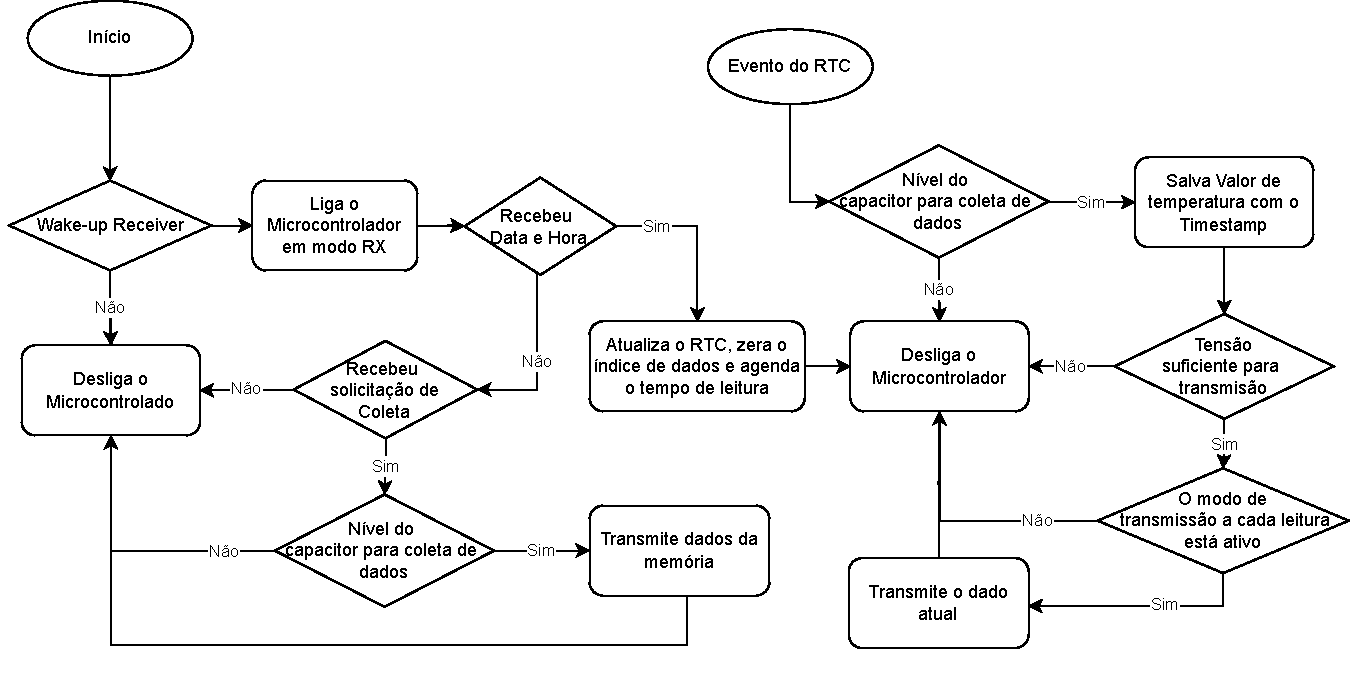
\includegraphics[scale=0.7]{img/fluxogramaOperacao.drawio.pdf}
  \end{center}
  \fonte{Elaborado pelo autor}
  \label{fig:fluxo}
\end{figure}
%%%%%\Floatbarrier

Um exemplo claro e notório deste tipo de avaliação se dá na inclusão de um bloco de verificação da tensão acumulada no capacitor de retenção. Com isso, se espera manter um nível mínimo de potência para manter o calendário do RTC ativo, visto que a interrupção de energia, zeraria o calendário.
Na Figura~\ref{fig:fluxo} pode-se ver a representação completa deste fluxo de operação. Além disso, se faz preciso a inclusão de um bloco para configuração inicial do sistema, já que informações anteriores precisam ser descartadas e isso pode ser feito simplesmente com o início de uma inserção da hora do sistema. Esta etapa de configuração está situada a esquerda do fluxograma. Uma vez que o sistema esteja iniciado, o RTC passa a gerenciar a alimentação do microcontrolador através de um intervalo de tempo previamente configurado. Ao ligar, a primeira função executada é a detecção de nível de tensão de alimentação. Caso haja energia suficiente para uma escrita na memória do microcontrolador, o pacote é montado juntamente com a informação de temperatura e \textit{Timestamp}. Caso o valor lido na tensão de alimentação seja suficiente para uma transmissão de rádio e o sistema esteja pre configurado para transmitir sempre, uma transmissão é realizada. Caso contrário, o microcontrolador corta a sua fonte de energia para aguardar um próximo evento do RTC. 
Quanto ao processo que descreve a etapa de configuração, sua ativação depende do sistema de \textit{Wake-up Receiver}, que ao ligar microcontrolador, coloca este em estado de escuta de rádio. Podendo a partir dai configurar a hora e data ou ativar o rádio para transmitir os pacotes armazenados na memória do microcontrolador.



%%%%%%%%%%%%%%%%%%%%%%%%%%%%%%%%%%%%%%%%%%%%%%%%%%%%%%%%%%%%%%%%%%%%%%
\section{Hardware}
%%%%%%%%%%%%%%%%%%%%%%%%%%%%%%%%%%%%%%%%%%%%%%%%%%%%%%%%%%%%%%%%%%%%%%
Após a modelagem apresentada no referencial teórico, torna-se possível especificar os requisitos do dispositivo eletrônico capaz de executar as operações citadas no fluxograma de operação da Figura~\ref{fig:fluxo}. Neste subcapítulo será detalhado cada parte do hardware proposto mostrado na Figura~\ref{fig:sistema}, considerando o dispositivo de colheita de energia e o \textit{"wake-up receiver"} como algo a ser acoplado ao sistema em um trabalho posterior.

\begin{figure}[h!]
  \caption{Diagrama de blocos dos componentes do hardware.}
  \begin{center}
      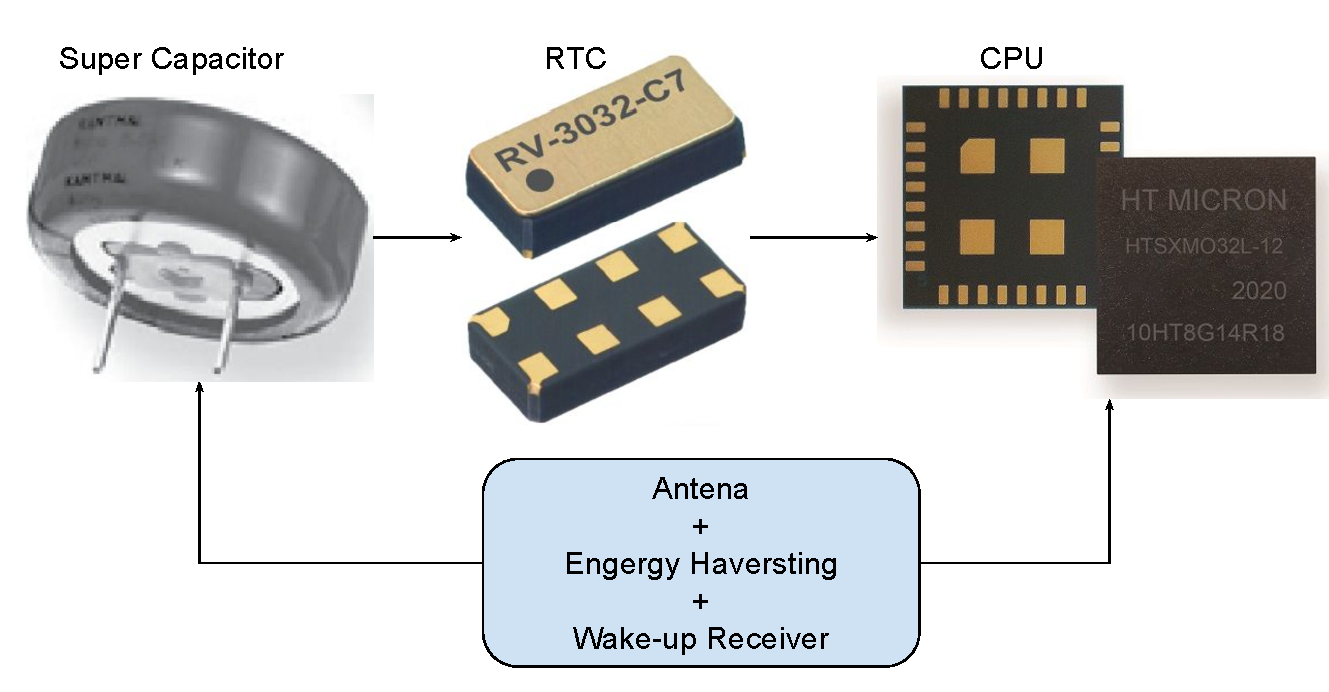
\includegraphics[scale=0.7]{img/sistema.pdf}
  \end{center}
  \fonte{Elaborado pelo autor}
  \label{fig:sistema}
\end{figure}
%%%%%\Floatbarrier
%%%%%%%%%%%%%%%%%%%%%%%%%%%%%%%%%%%%%%%%%%%%%%%%%%%%%%%%%%%%%%%%%%%%%%
\subsection{RTC}\label{sec:RTC}
%%%%%%%%%%%%%%%%%%%%%%%%%%%%%%%%%%%%%%%%%%%%%%%%%%%%%%%%%%%%%%%%%%%%%%
Aplicações de monitoramento de temperaturas em dispositivos IoT muitas vezes podem contar com a definição de hora e data baseados no momento da transmissão, sendo dispensável a estes o uso de circuitos com \textit{Real Time Clock}(RTC), relógios de tempo real~\cite{Soh}. Nos casos em que a janela de transmissão de dados ocorre em momentos distintos da coleta dos mesmos, uma marcação de tempo se faz necessária para garantir a procedência desta coleta.

Para garantir essa marcação de tempo neste projeto, procurou-se obter um circuito de RTC capaz de manter sua funcionalidade por longos períodos de tempo com um consumo mínimo de potência. Dentre as soluções pesquisadas, cabe um destaque especial para o RV-3032~\cite{rtc} da empresa \textit{Micro Crystal} que combina um circuito integrado (CI) do tipo CMOS com um cristal ressonador interno. 

Este RTC funciona sob vácuo em embalagem cerâmica hermeticamente fechada com tampa metálica. Seu consumo de corrente em operação chega a níveis consideravelmente baixos, da ordem de nano amperes (nA). Além disso, o mesmo possuis uma compensação da precisão em função da temperatura (TXCO), que garante uma precisão de $\pm$2,5~ppm em toda a faixa de -40~$^o$C até 85~$^o$C.

\begin{figure}[h!]
  \caption{Curva de operação do RV-3032}
  \begin{center}
      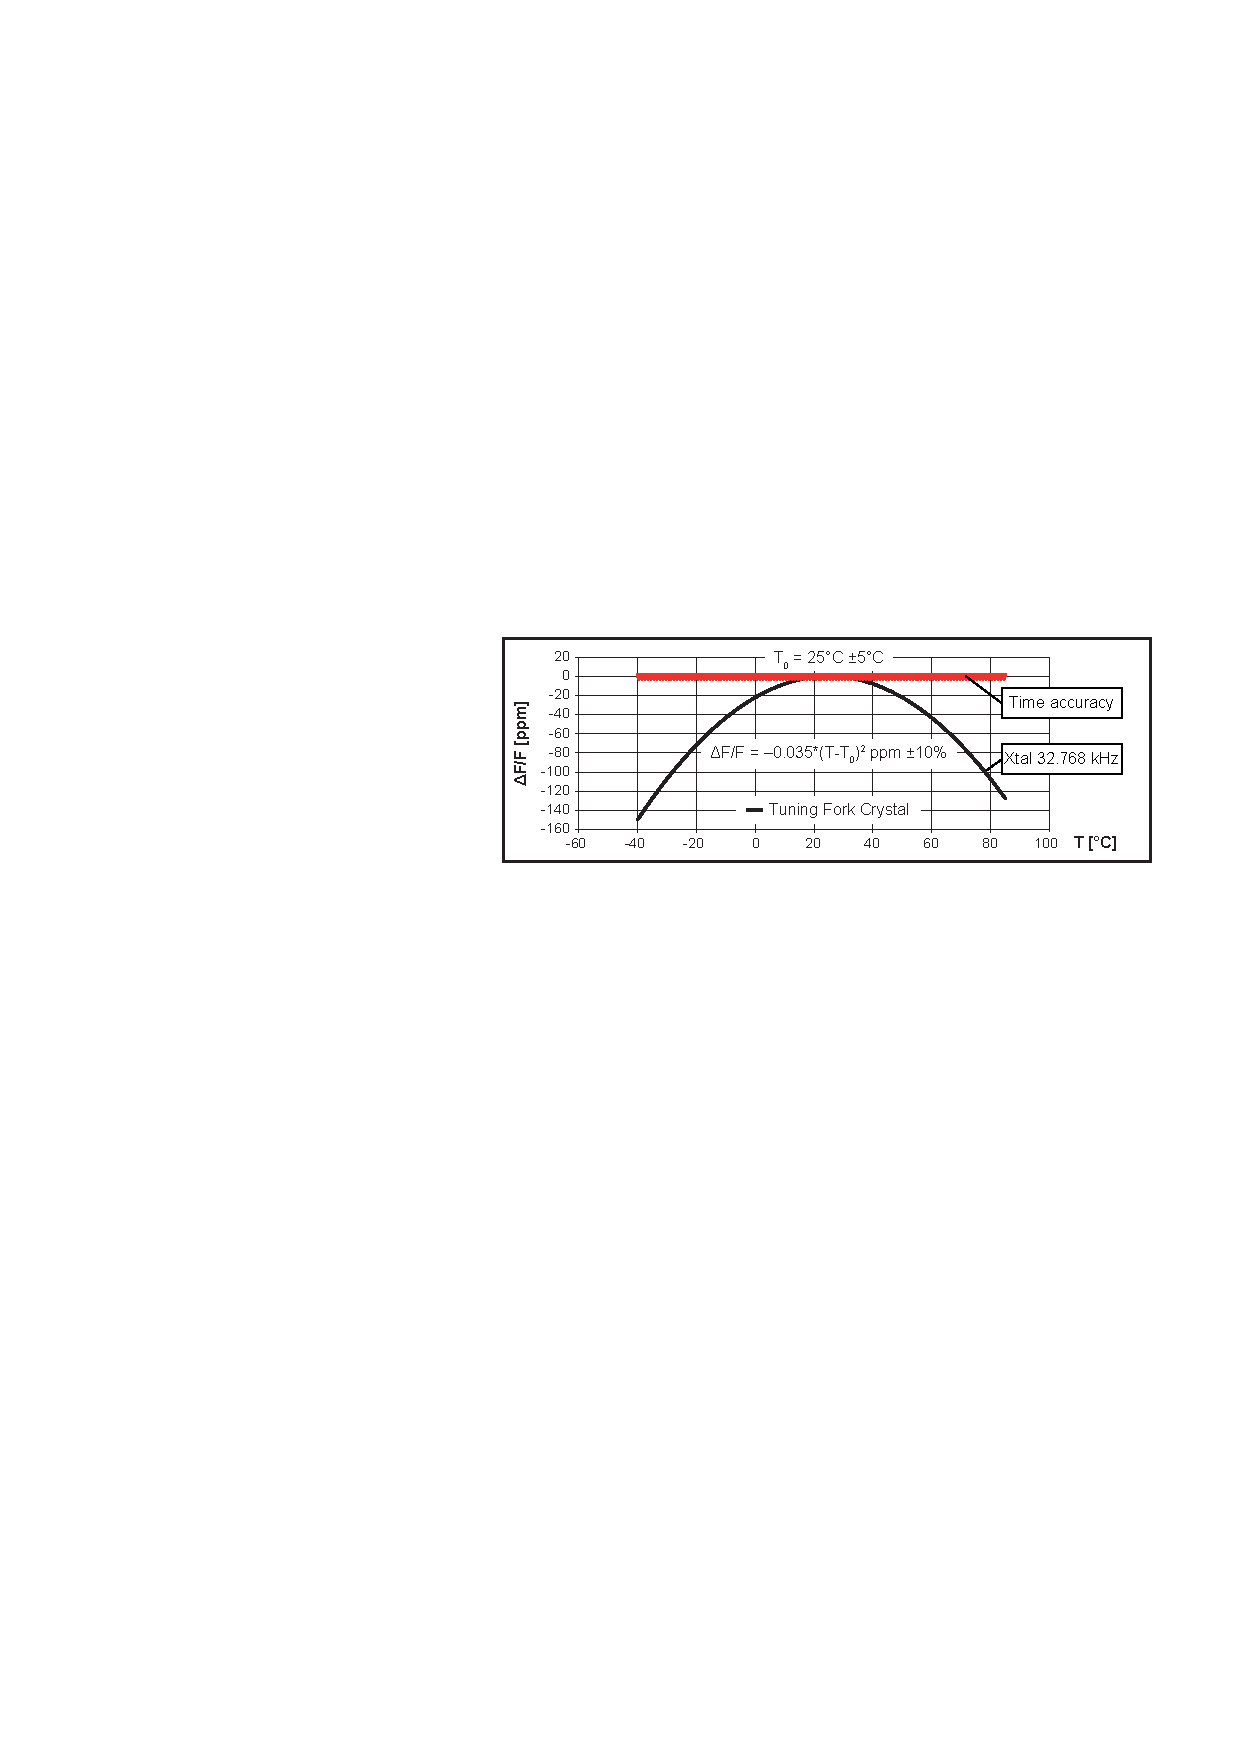
\includegraphics[scale=0.8]{img/RTCcurva.pdf}
  \end{center}
  \fonte{\citeonline{rtc}}
  \label{fig:RTC}
\end{figure}
%%%%%\Floatbarrier
A inserção de um sensor de temperatura e do cristal dentro do RV-3032 além de aumentar a precisão fora da temperatura convencional de 25~$^o$C, possibilita o uso desta informação de temperatura para dispositivos IoT que possam fazer esse tipo de aquisição.
Este sensor possui uma acurácia típica de $\pm$ 1~$^o$C que é relativamente alta, mas que não apresenta prejuízos para o estudo proposto, uma vez que a temperatura aproximada se faz suficiente para este controle. Ademais, existe uma região de memória onde se pode efetuar calibragens para garantir a acurácia.
Outra vantagem do uso deste RTC nesta aplicação, se dá em função da possibilidade de configuração de alarmes capazes de acordar o processador por uma janela de tempo preestipulada, ou o cruzamento por uma temperatura específica. Esta função, pode ser considerada um real diferencial para a redução do consumo de operação do dispositivo, já que permite ao microcontrolador ligado ao RTC entrar em um modo profundo de economia de energia (\textit{Deep Sleep Mode}).

%%%%%%%%%%%%%%%%%%%%%%%%%%%%%%%%%%%%%%%%%%%%%%%%%%%%%%%%%%%%%%%%%%%%%%
\subsection{Super capacitor}\label{sec:supercap}
%%%%%%%%%%%%%%%%%%%%%%%%%%%%%%%%%%%%%%%%%%%%%%%%%%%%%%%%%%%%%%%%%%%%%%
Em um estudo realizado por \citeonline{supercap}, concluiu-se que o uso de super capacitores em sistemas de coleta de energia por RF pode ser uma alternativa razoável, pois embora eles possuam uma densidade de acúmulo de carga centenas de vezes menores que baterias, eles se mostram eficientes em situações de carga e descarga. Neste mesmo artigo, de acordo com o autor, mediu-se o tempo de carga de um capacitor de 3~F sendo notado um tempo de aproximadamente três horas para um dispositivo comercial de conversão de energia.

Para avaliar a curva de carga e descarga do capacitor, tem-se que considerar os princípios básicos deste componente, como a relação \textit{RC} também chamada de constante de tempo ($\tau$). Na Tabela~\ref{tb:capacitor} estes valores são apresentados e a partir deles, pode-se obter a curva apresentada na Figura~\ref{fig:capacitor}.

% Please add the following required packages to your document preamble:
% \usepackage{booktabs}
\begin{table}
\begin{center}
\caption{Valores de $\tau$.}
\label{tb:capacitor}
\begin{tabular}{@{}cccc@{}}
\toprule
 & \textbf{$t$}  &\textbf{ $v(t)/V_0$} & \\ \midrule
 & $1\tau$ & $0,36788$ & \\
 & $2\tau$ & $0,13534$ & \\
 & $3\tau$ & $0,04979$ & \\
 & $4\tau$ & $0,01832$ & \\
 & $5\tau$ & $0,00674$ & \\ \bottomrule
\end{tabular}
\end{center}  
\fonte{Adaptado de \citeonline[p.~246]{Alexander2013}}
\end{table}

\begin{figure}[h!]
  \caption{Curva de carga característica de um capacitor.}
  \begin{center}
      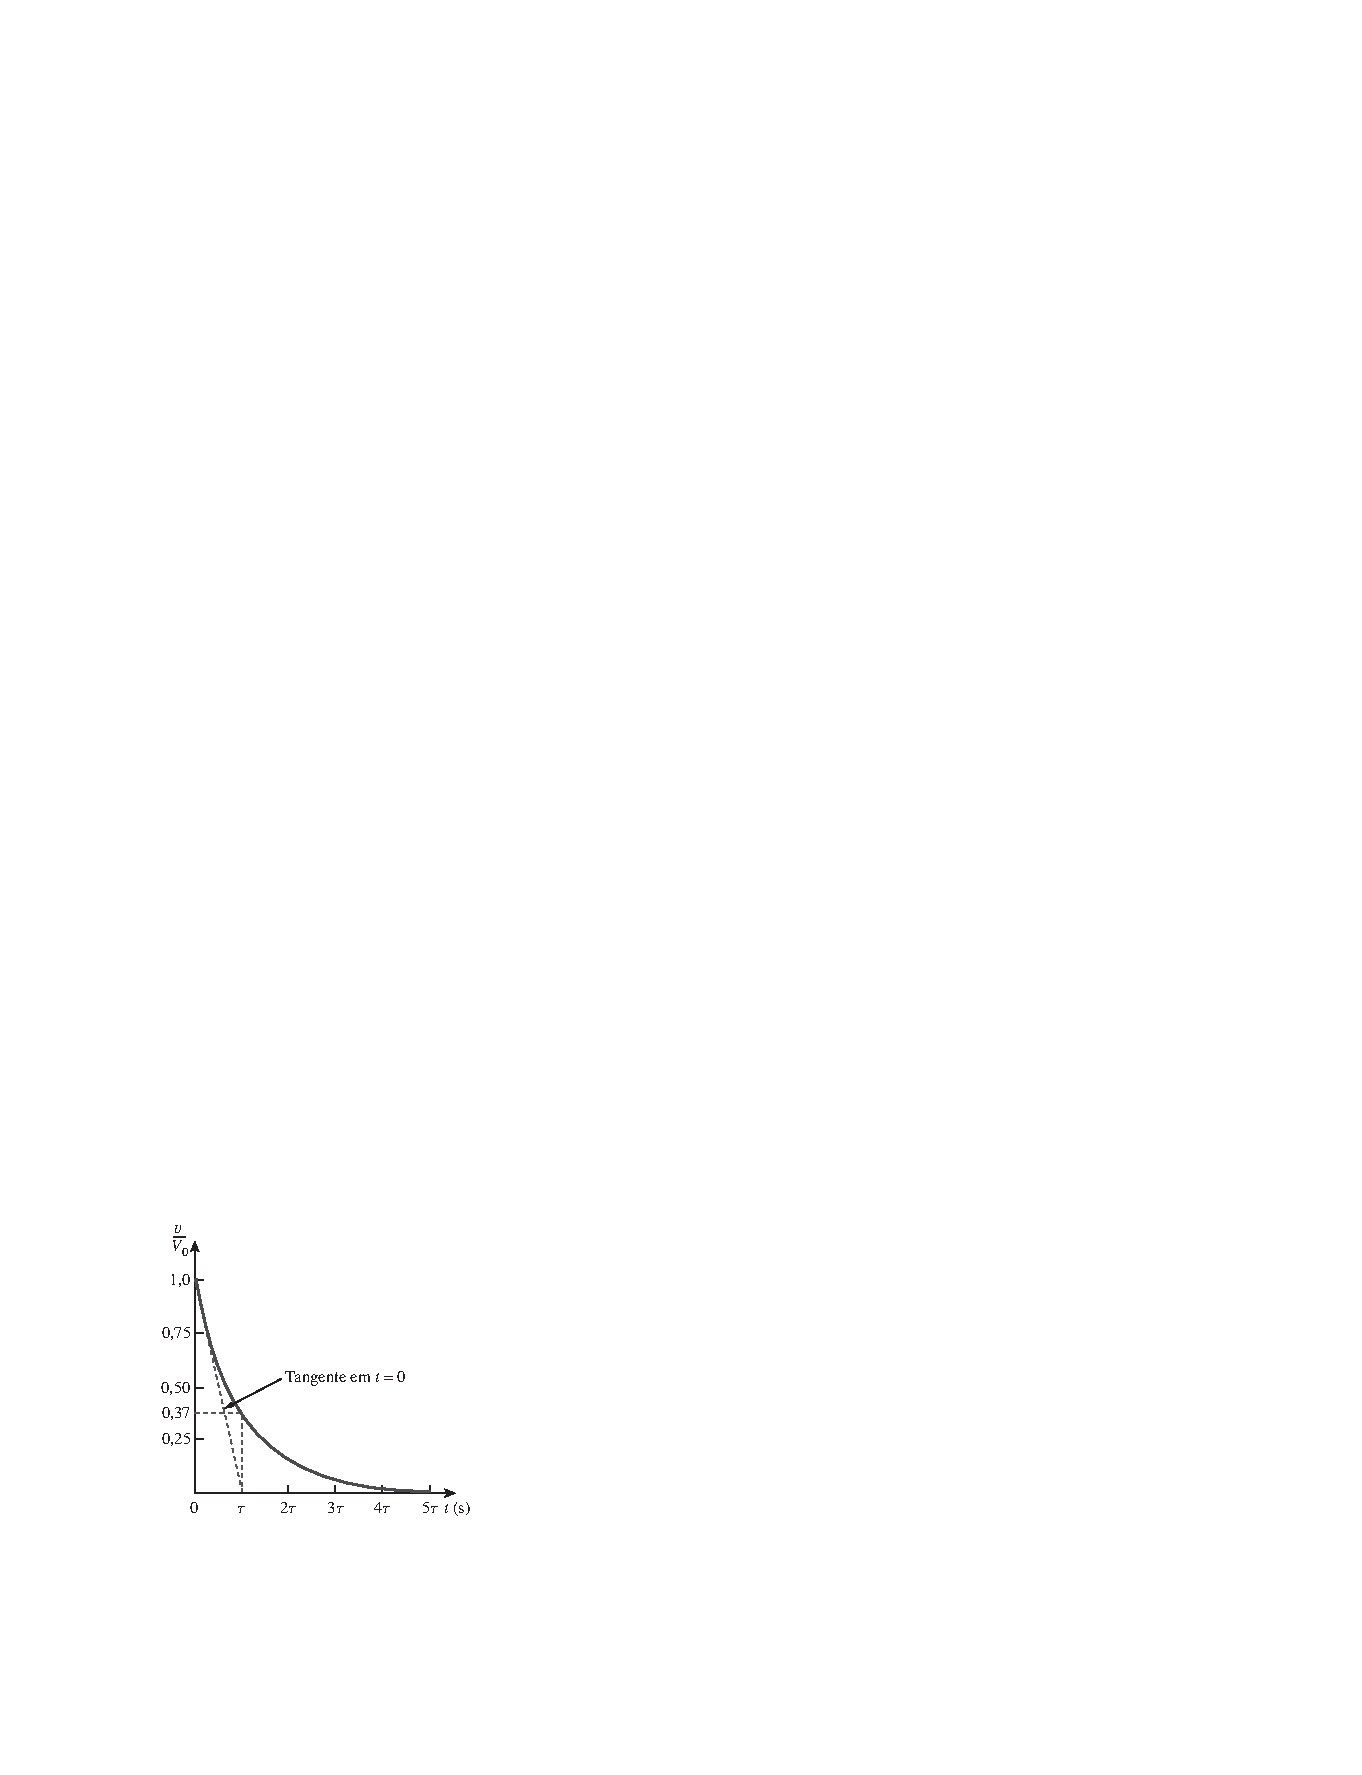
\includegraphics[scale=1]{img/capacitor.pdf}
  \end{center}
  \fonte{\citeonline[p.~246]{Alexander2013}}
  \label{fig:capacitor}
\end{figure}
%%%%%\Floatbarrier

Já para estimar o valor ideal de capacitor a ser empregado nesta solução, considerou-se a corrente máxima de \IRTC do RTC conforme as informações do datasheet citado no tópico RTC~\ref{sec:RTC}. A partir disso, e considerando o range de tensão de operação ente \VminRTC a \VmaxRTC, obteve-se inicialmente o delta de tensão de operação através da equação~\ref{eq:dv}.

\begin{equation}
    \Delta V = V_{cc}-V_{min}
  \label{eq:dv}
\end{equation}


Onde $V_{cc}$ é a tensão de entrada e $V_{min}$ é a tensão mínima de operação do RTC.

\begin{equation}
     \Delta V =\VmaxRTC-\VminRTC = \VdeltaRTC
\end{equation}

A partir da equação do tempo de descarga, pode-se obter o valor do capacitor considerando um tempo de retenção de aproximadamente 40~dias. Estipulou-se um tempo demasiado alto para garantir longos períodos de tempo sem o recebimento de energia através do sistema de colheita. A equação~\ref{eq:T} define o cálculo do tempo e transformando na equação~\ref{eq:C} calcula-se o valor capacitor.


\begin{equation}
    T=\frac{\Delta V \times C}{I}
  \label{eq:T}
\end{equation}

Onde $T$ é o tempo em segundos, $\Delta V$ é a variação da tensão de operação do RTC, $I$ é a corrente de operação do RTC e $C$ é o capacitor a ser calculado.

\begin{equation}
    C=\frac{(40~Dias\times 60\times60\times24) \times \IRTC}{3,7V} = 224mF \cong \Cap
      \label{eq:C}
\end{equation}

O capacitor foi aproximado para um valor comercial e após uma busca em distribuidores de componentes, escolheu-se pelo \textit{Part Number} LM055224A~\cite{Ohmite} baseado na baixa fuga de corrente e na disponibilidade no mercado nacional.

%%%%%%%%%%%%%%%%%%%%%%%%%%%%%%%%%%%%%%%%%%%%%%%%%%%%%%%%%%%%%%%%%%%%%%
\subsection{Microcontrolador do rádio HT32SX}\label{sc:HT32SX}
%%%%%%%%%%%%%%%%%%%%%%%%%%%%%%%%%%%%%%%%%%%%%%%%%%%%%%%%%%%%%%%%%%%%%%
Para a escolha do microcontrolador, utilizou-se como referência o primeiro SiP equipado com rádio Sigfox fabricado no mercado nacional brasileiro pela empresa HT Micron. O iMCP–HT32SX é um circuito integrado multicomponente (MCO) projetado para fornecer uma solução de conectividade pronta para uso para aplicativos de Internet das Coisas (IoT). Ele fornece comunicações de uplink (transmissão) e downlink (recepção), e é o primeiro produto HT Micron em uma nova família de componentes. Suas pequenas dimensões, alto desempenho e baixo consumo de energia visam a melhor experiência para desenvolvedores de IoT. Possui um ARM Cortex M0+ de 32 bits (STM32L052x8) e o transceptor de baixa potência S2-LP (12~dBm) da ST Microelectronics combinado com o SKY66420 da Skyworks Solutions montado em um único chip. Este chip possui também uma EEPROM com capacidade para armazenar 2k Bytes. Na Figura~\ref{fig:blockHT32SX} pode-se ver o diagrama de blocos do iMCP-HT32SX desenvolvido pela empresa HT Micron.

\begin{figure}[h!]
  \caption{Diagrama de blocos do iMCP–HT32SX.}
  \begin{center}
      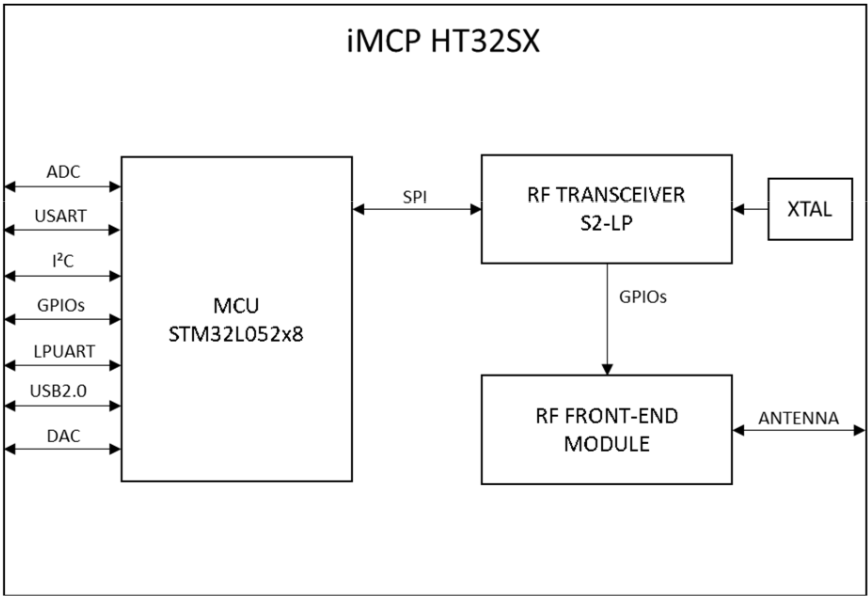
\includegraphics[scale=0.5]{img/imcpHT32sx.png}
  \end{center}
  \fonte{HT Micron\cite{HTSXMO32L} }
  \label{fig:blockHT32SX}
\end{figure}
%%%%%\Floatbarrier

Além dos requisitos já citados, o HT32SX ainda conta com um sensor de temperatura interno, que poderia ser utilizado para o obter este dado e assim traçar a curva desta. Porém, devido a disponibilidade de um sensor de temperatura dentro do RTC, optou-se por utilizar este e assim evitar a retirada do modo profundo de economia de energia do microcontrolador para executar esta tarefa.
%%%%%%%%%%%%%%%%%%%%%%%%%%%%%%%%%%%%%%%%%%%%%%%%%%%%%%%%%%%%%%%%%%%%%%
\subsection{HTSXMO32L-22}
%%%%%%%%%%%%%%%%%%%%%%%%%%%%%%%%%%%%%%%%%%%%%%%%%%%%%%%%%%%%%%%%%%%%%%
A mesma empresa HT Micron disponibiliza um kit de desenvolvimento para testar o HT32SX. A Placa de Avaliação iMCP HTSXMO32L-22 foi projetada para facilitar o primeiro contato de novos usuários com o iMCP HT32SX, além de fornecer ao usuário avançado a possibilidade de começar a programar e desenvolver produtos imediatamente com estrutura mínima. Todos os recursos do HT32SX estão disponíveis na placa de avaliação e o esquema elétrico pode ser visto no Anexo~\ref{ax:esquemaHT}. Duas opções de alimentação podem ser usadas: conexão USB ou bateria externa. A placa de avaliação muda automaticamente para alimentação USB quando esta estiver disponível, possibilitando praticidade na validação do software em fase de testes. Na Figura~\ref{fig:placaHT32SX} pode-se ver a Placa iMCP HTSXMO32L-22 desenvolvida pela empresa HT Micron na versão 2.0.

\begin{figure}[h!]
  \caption{Placa iMCP HTSXMO32L-22.}
  \begin{center}
      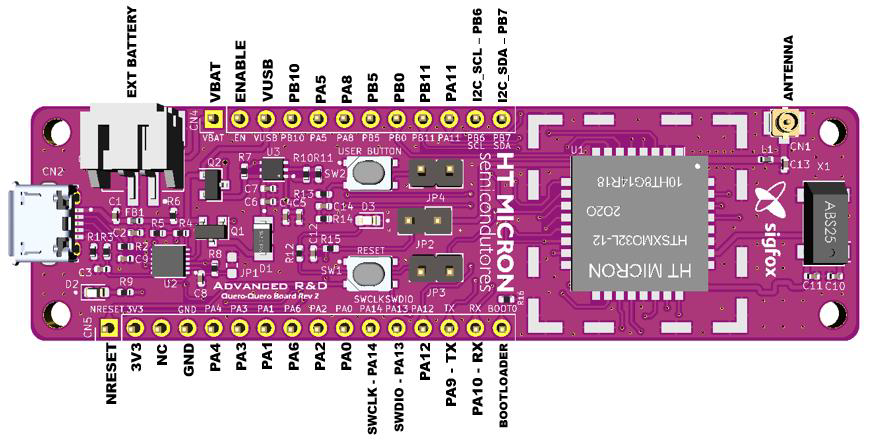
\includegraphics[scale=0.5]{img/placa.png}
  \end{center}
  \fonte{HT Micron\cite{HTSXMO32L} }
  \label{fig:placaHT32SX}
\end{figure}
%%%%%\Floatbarrier

A conexão para bateria externa torna a placa de avaliação portátil, facilitando testar a conectividade do Sigfox em qualquer lugar que se vá. Como mencionado na seção~\ref{sc:HT32SX}, a substituição de baterias por um super capacitor se fará presente nesta conexão. Os barramentos laterais possibilitam acesso direto aos pinos de entradas e saídas. Com isso, a integração entre as diferentes partes do protótipo inicial pode ser efetuada sem necessidade de modificações complexas.

Como se espera uma utilização mínima de espaço nesta aplicação, o uso de antena externa será feito inicialmente. Uma vem que a solução apresente resultado favorável, esta pode ser alterada para uma antena de circuito impresso juntamente com a integração de todos os recursos de hardware. 
%%%%%%%%%%%%%%%%%%%%%%%%%%%%%%%%%%%%%%%%%%%%%%%%%%%%%%%%%%%%%%%%%%%%%%
\subsection{Esquema elétrico\label{sec:esquematico}}
%%%%%%%%%%%%%%%%%%%%%%%%%%%%%%%%%%%%%%%%%%%%%%%%%%%%%%%%%%%%%%%%%%%%%%
De forma a diminuir ao máximo os impactos da corrente de operação do iMCP HTSXMO32L-22, optou-se por uma abordagem onde o RTC torna-se o responsável pelo ligamento deste. Sendo assim, produziu-se um diagrama elétrico onde uma chave digital pode ligar e desligar a alimentação do módulo com o microcontrolador. Esta chave por sua vez, está ligada à saída de interrupção do RTC. Uma vez que esta chave digital seja acionada e o microcontrolador esteja ligado, o mesmo mantém uma trava paralela para esta chave, controlada por um de seus pinos de GPIO, até que as operações descritas no fluxograma da Figura~\ref{fig:fluxo} sejam executadas e por fim ocorre uma liberação deste pino de GPIO para cortar totalmente a alimentação de energia do circuito com o microcontrolador.


\begin{figure}[h!]
  \caption{Esquema elétrico - RTC.}
  \begin{center}
      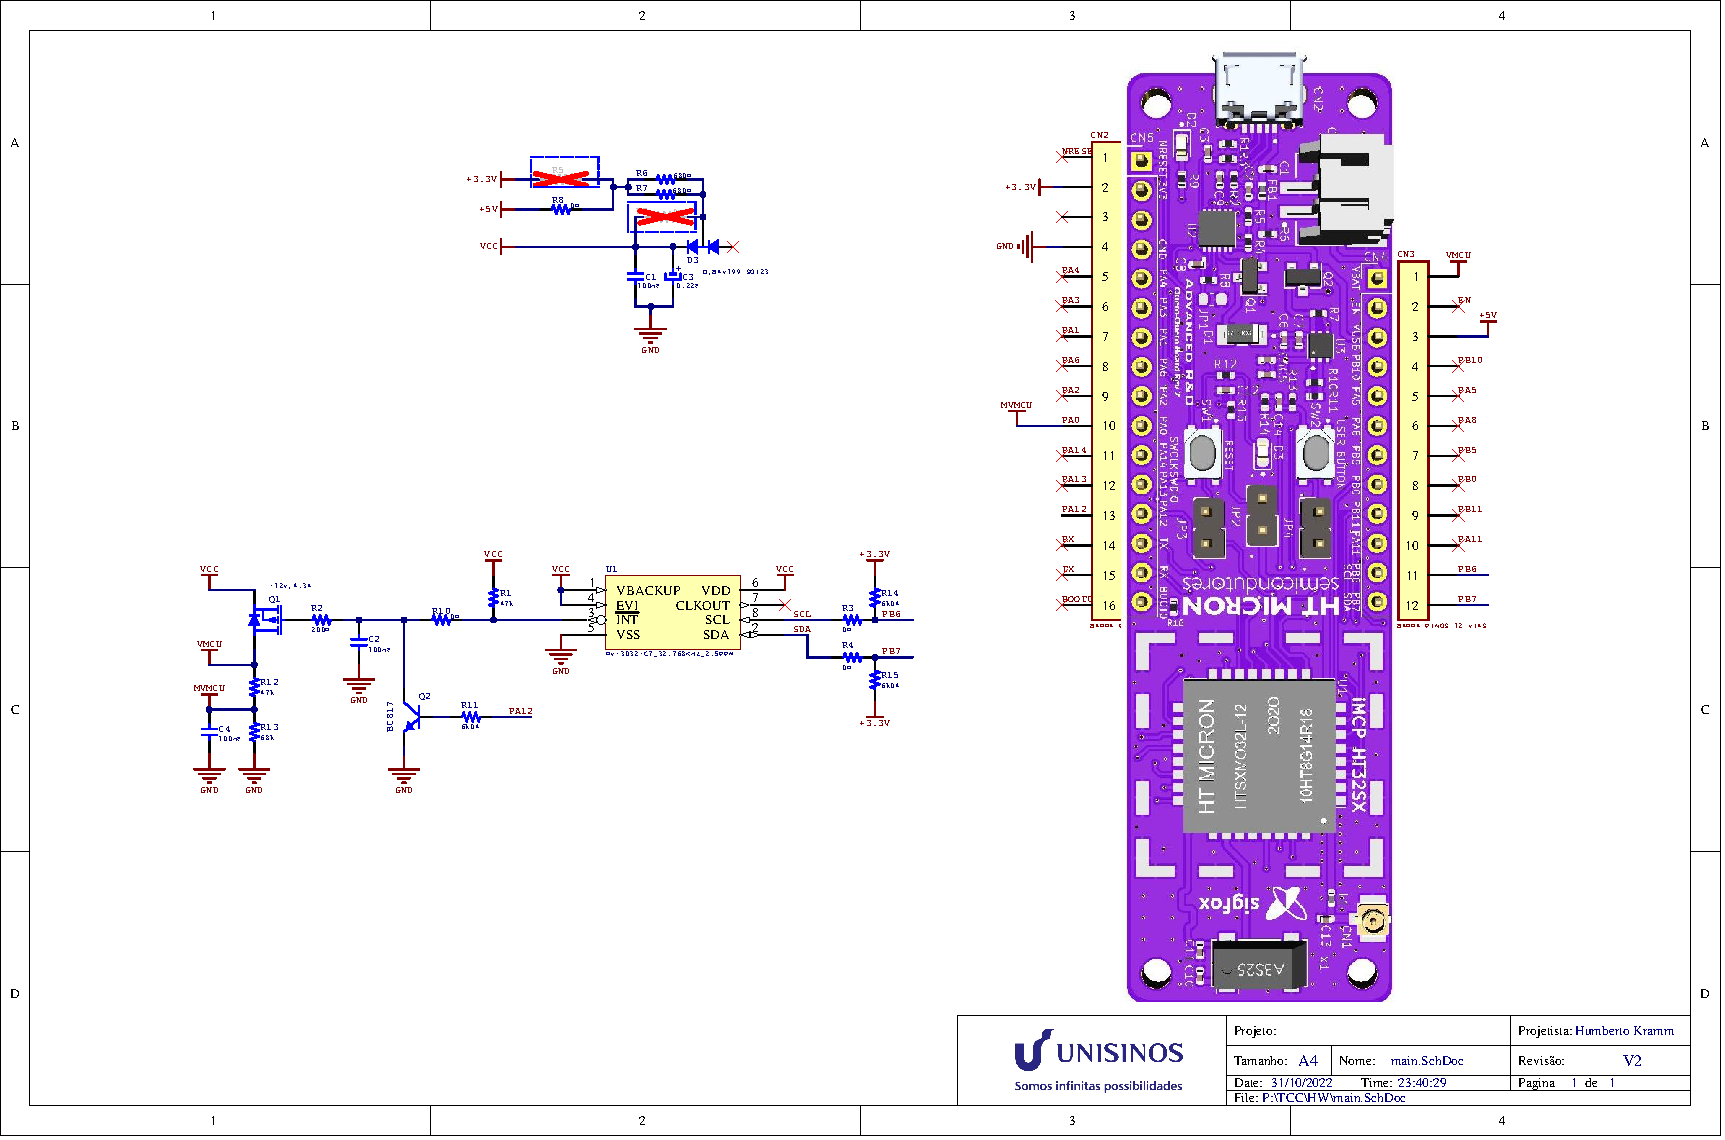
\includegraphics[scale=1.2,
      %trim={<left> <lower> <right> <upper>} 
      trim={3cm 5cm 13cm 9cm},
      clip]{esquemas/PTH TCC-RTC V2.PDF}
  \end{center}
  \fonte{Elaborado pelo autor}
  \label{fig:esquemaEle}
\end{figure}
%%%%%\Floatbarrier

Na Figura~\ref{fig:esquemaEle} pode-se ver este circuito com uma menção especial para o transistor $Q1$ que faz o papel da chave digital que mantel a alimentação para o módulo e o transistor $Q2$ que mantem essa chave ligada através do pino de GPIO PA12 do iMCP HTSXMO32L-22. Além disso, junto ao $Q1$, pode-se ver os resistores $R12$ e $R13$ que formam um circuito divisor de tensão com impedância relativamente alta para monitorar a tensão armazenada no super capacitor e determinar se há condições energéticas para efetuar as operações do fluxograma da Figura~\ref{fig:fluxo}.

No diagrama elétrico também está disposto o circuito com a conexão do super capacitor, já montado com um diodo de baixa fuga para impedir a descarga do capacitor pelo circuito de carga e resistores em série para limitar a corrente de carga deste. Também deixou-se conexões alternativas através do resistor $R5$ e  $R9$ para flexibilizar o circuito em outros modos de operação não previstos. Este circuito está apresentado na Figura~\ref{fig:esquemaElecap}.

\begin{figure}[h!]
  \caption{Esquema elétrico - Circuito do capacitor.}
  \begin{center}
      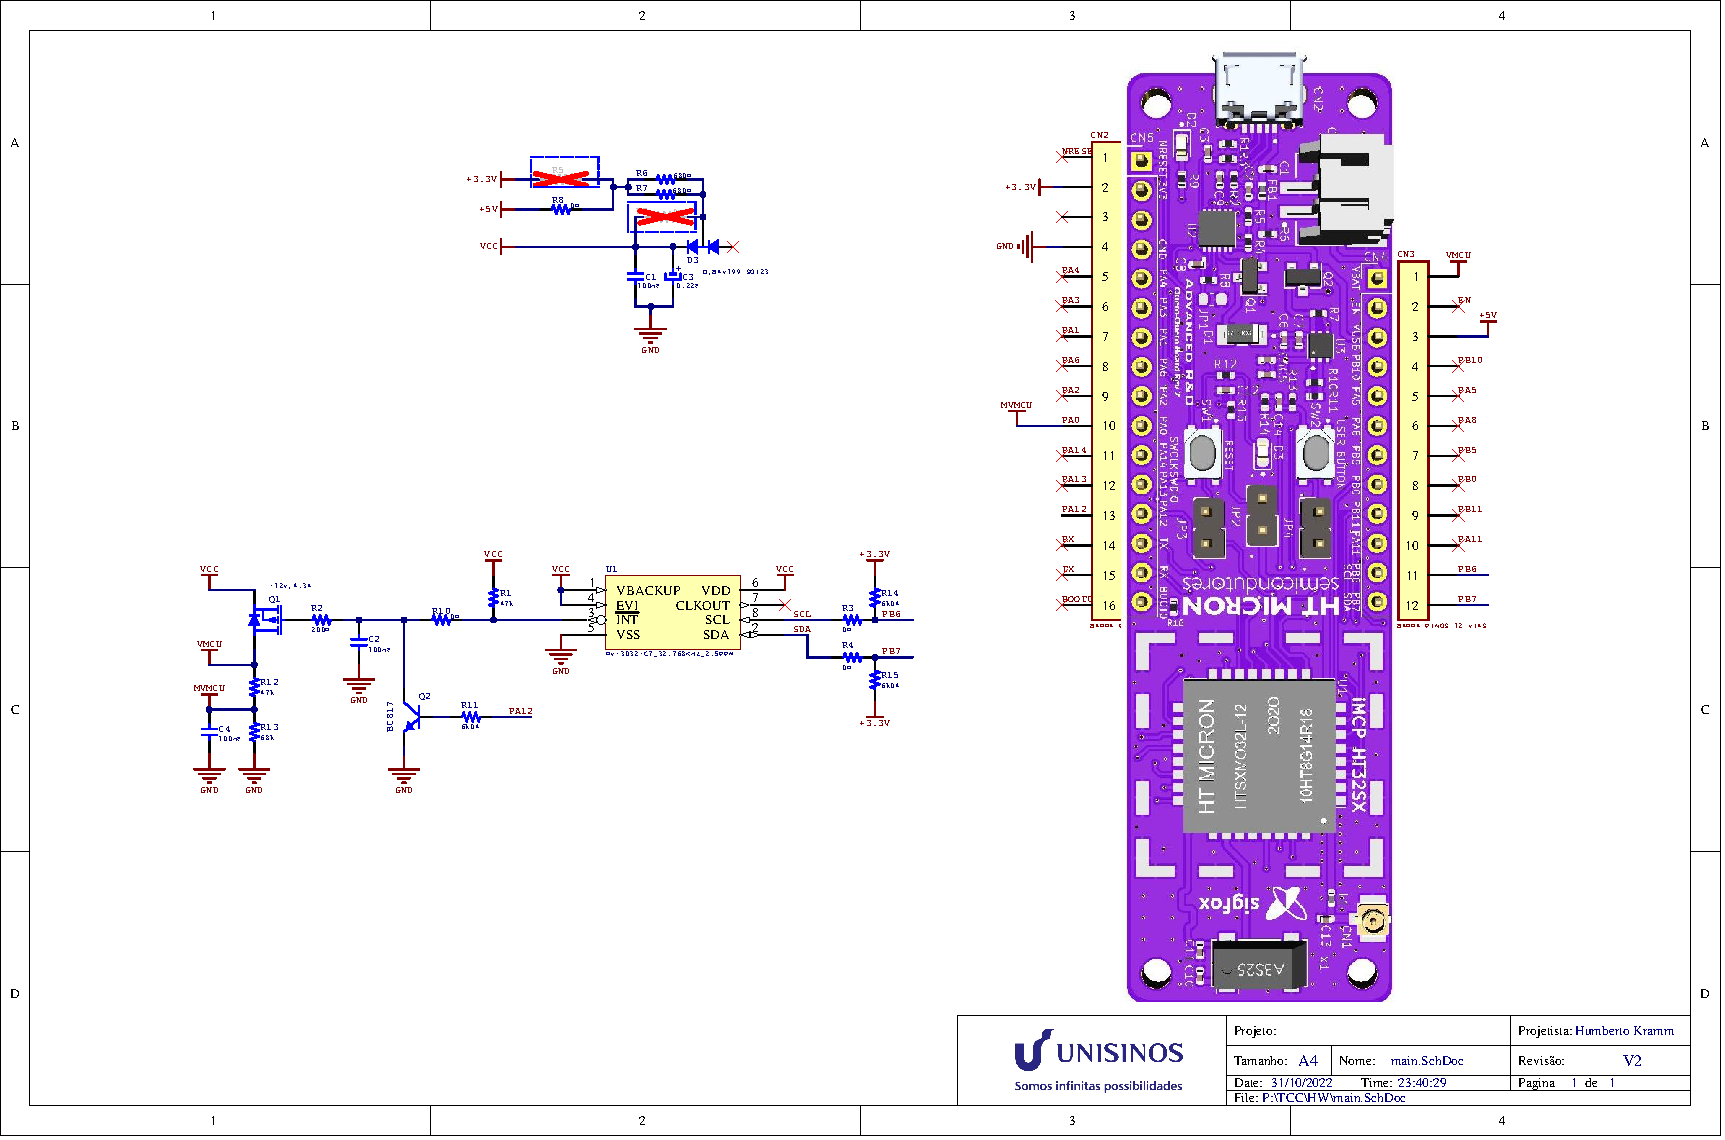
\includegraphics[scale=1.2,
      %trim={<left> <lower> <right> <upper>} 
      trim={7cm 13cm 16cm 2cm},
      clip]{esquemas/PTH TCC-RTC V2.PDF}
  \end{center}
  \fonte{Elaborado pelo autor}
  \label{fig:esquemaElecap}
\end{figure}
%%%%%\Floatbarrier

Nestas condições, pode-se executar uma análise detalhada do tempo de carga do capacitor e assim determinar o tempo necessário para atingir um patamar suficiente de energia para as operações normais do sistema. Na Figura~\ref{fig:capcargaP} está representada esta curva com algumas sinalizações no gráfico indicando os tempos para se atingir os percentuais característicos de carga comuns a capacitores.

\begin{figure}
  \caption{Curva prática de carga do capacitor.}
  \begin{center}
      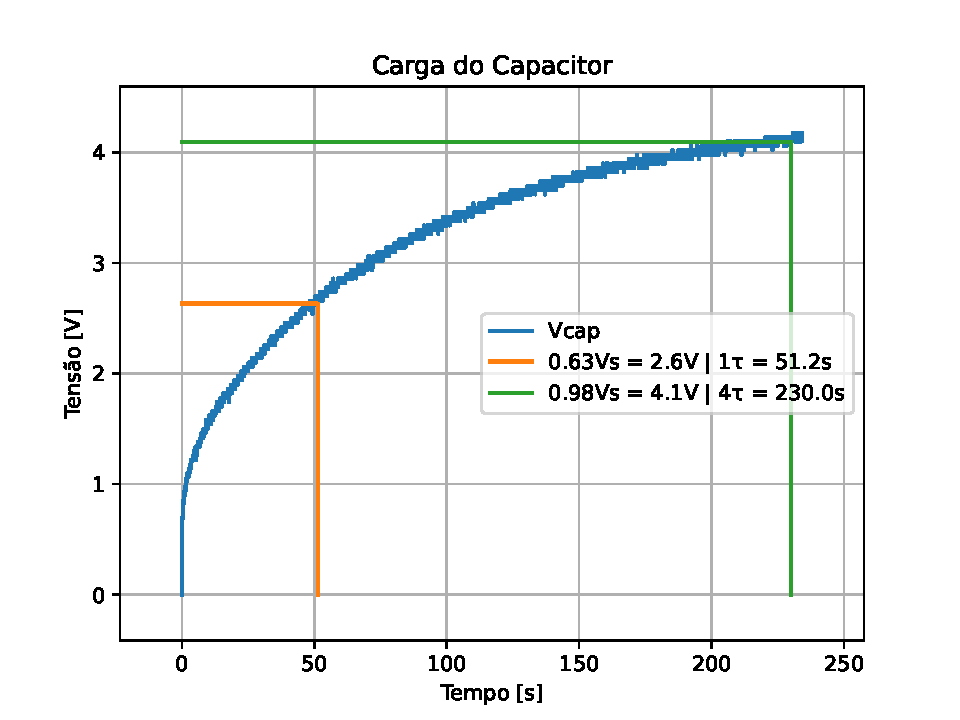
\includegraphics[scale=0.7]{scripts/supercapCarga.csv.pdf}
  \end{center}
  \fonte{Elaborado pelo autor}
  \label{fig:capcargaP}
\end{figure}

Vale destacar no gráfico da Figura~\ref{fig:capcargaP} que o tempo necessário para atingir boa parte da tensão máxima (4 $\tau$) é de aproximadamente 230~s e 50~s para atingir os 63~\% referentes as 1 $\tau$. A obtenção desta curva executou-se de forma prática considera apenas o RTC ligado ao sistema, desprezando a corrente necessária para o módulo iMCP HTSXMO32L-22, uma vez que este encontrava-se desenergizado pela através da chave digital.

Este tempo de carga está relacionado diretamente ao modelo de conexão inicial deste projeto, onde a alimentação principal do sistema é proveniente de uma conexão USB genérica, sendo limitada apenas pela corrente dos resistores $R6$ e $R7$ em série com o super capacitor. Posteriormente este circuito deve ser substituído pelo sistema de colheita de energia de ondas de rádio.
%%%%%%%%%%%%%%%%%%%%%%%%%%%%%%%%%%%%%%%%%%%%%%%%%%%%%%%%%%%%%%%%%%%%%%
\subsection{Placa de circuito impresso\label{sec:pcb}}
%%%%%%%%%%%%%%%%%%%%%%%%%%%%%%%%%%%%%%%%%%%%%%%%%%%%%%%%%%%%%%%%%%%%%%
A confecção da placa de circuito impresso se executou em um fabricante localizado na China, já a montagem dos componentes na placa foi executada manualmente pelo autor. Como é de se esperar, algumas etapas testadas do circuito se alteraram conforme os testes práticos do circuito se desenvolveram. Estas alterações já estão inclusas no esquema elétrico apresentado na seção~\ref{sec:esquematico}. Porém, devido ao tempo e custo adicional de um novo protótipo, estas alterações foram implementas através de cortes em trilhas, soldagem alternativa de componentes com uso de fios externos conectando as novas ligações. Estas ligações podem ser vistas na Figura~\ref{fig:fotoplaca} já acoplada na placa de desenvolvimento iMCP HTSXMO32L-22.


\begin{figure}[h!]
  \caption{Placa de circuito impresso na versão 1 com correções da versão 2.}
  \begin{center}
      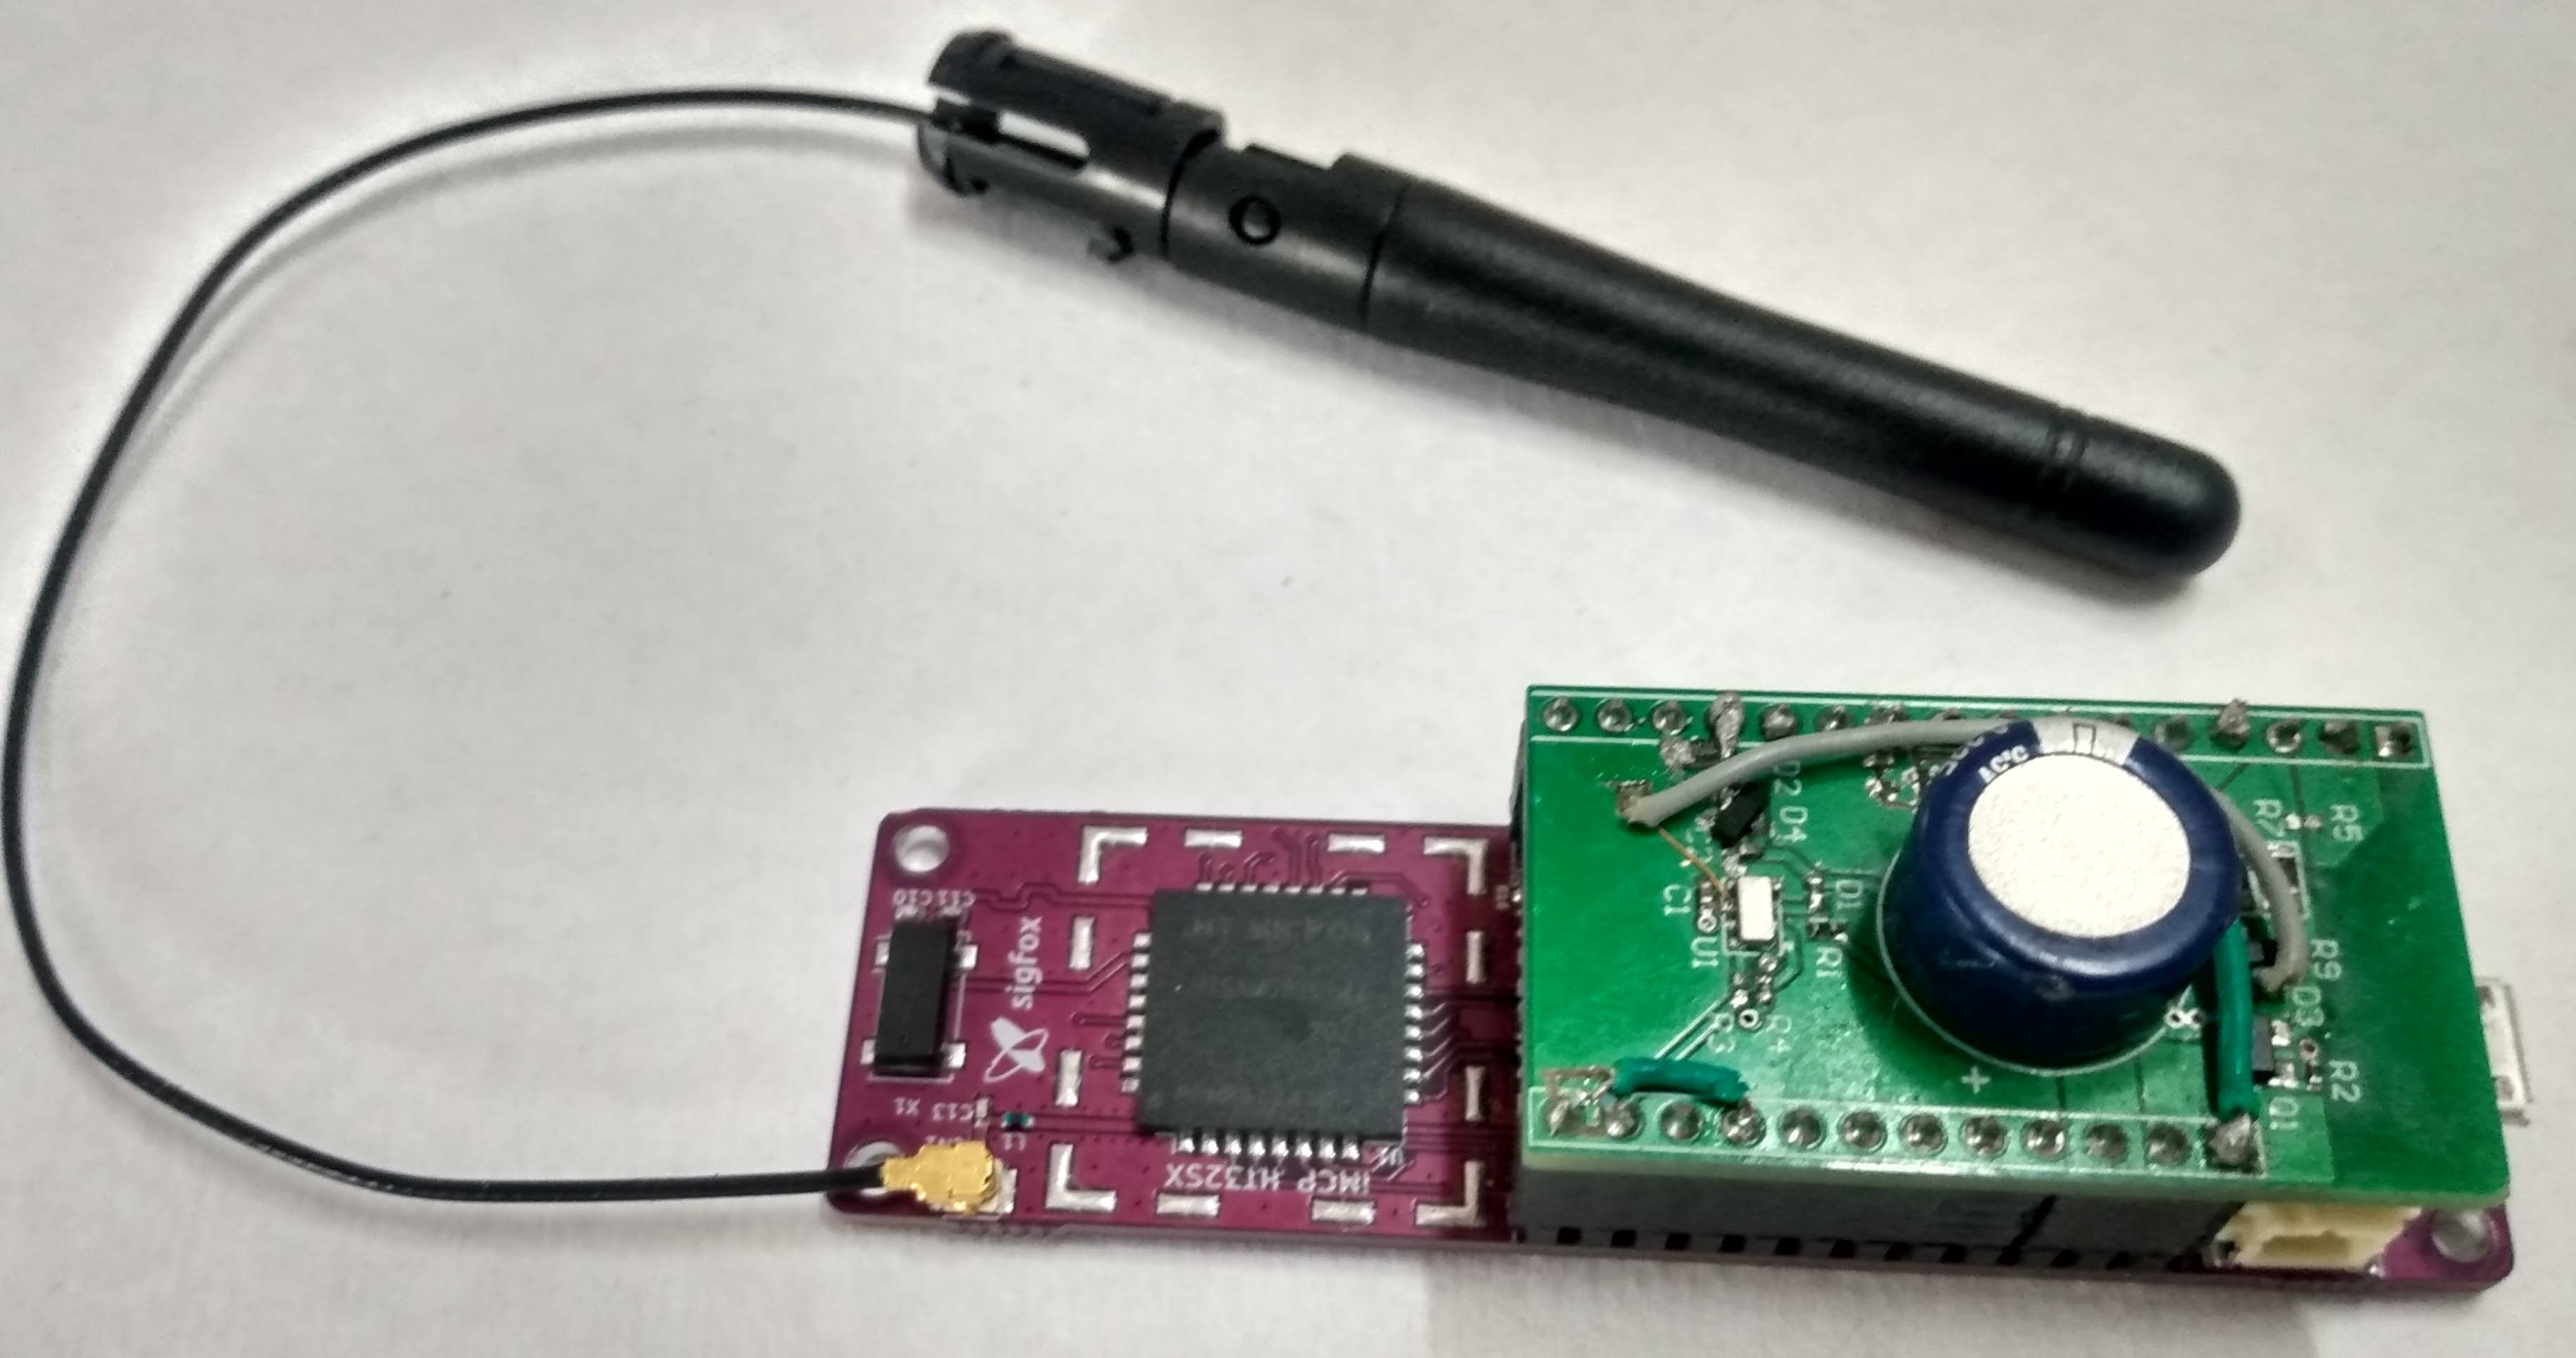
\includegraphics[scale=0.1]{img/fotoplaca.png}
  \end{center}
  \fonte{Elaborado pelo autor}
  \label{fig:fotoplaca}
\end{figure}
%%%%%\Floatbarrier

Assim como as alterações da versão 2 entraram na documentação de esquema elétrico, as alterações da placa de circuito impresso (PCI) foram igualmente corrigidas e uma versão virtualizada desta placa pode ser vista na Figura~\ref{fig:pcbV2} com os novos componentes e conexões remapeadas e roteadas. Pode-se ver que diferentemente do que ocorre na Figura~\ref{fig:fotoplaca}, onde as conexões para barras de pinos estão instaladas em um lado da placa que privilegiam o acesso à depuração nos testes, a versão virtualizada apresenta a montagem no lado esperado para testes futuros protegendo as ligações elétricas com a cobertura da outra placa e aproveitando melhor o espaço necessário.

\begin{figure}[h!]
  \caption{Placa de circuito impresso montada virtualmente na versão 2.}
  \begin{center}
      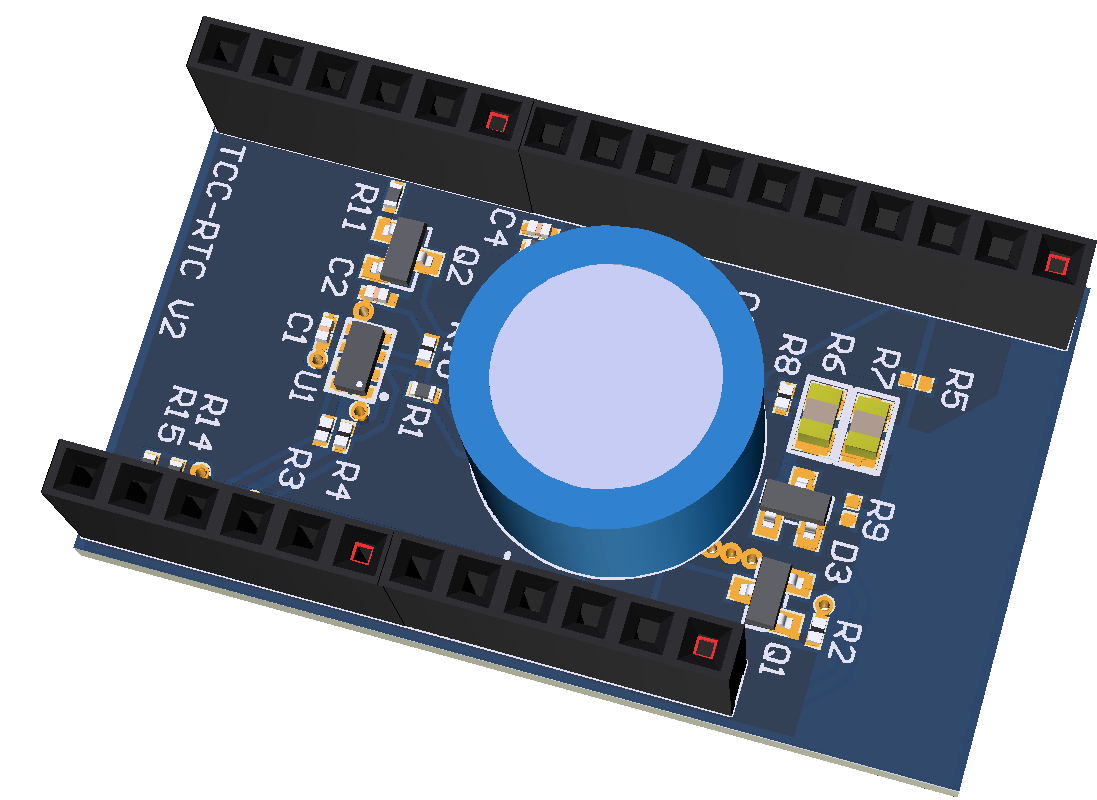
\includegraphics[scale=0.5]{img/PCB_TCC.png}
  \end{center}
  \fonte{Elaborado pelo autor}
  \label{fig:pcbV2}
\end{figure}
%%%%%\Floatbarrier




%%%%%%%%%%%%%%%%%%%%%%%%%%%%%%%%%%%%%%%%%%%%%%%%%%%%%%%%%%%%%%%%%%%%%%
\section{\textit{Software}}\label{sec:software}
%%%%%%%%%%%%%%%%%%%%%%%%%%%%%%%%%%%%%%%%%%%%%%%%%%%%%%%%%%%%%%%%%%%%%%
Após a modelagem, deve-se implementar o modelo de software baseado nos levantamentos do fluxograma de operação mostrado na Figura~\ref{fig:fluxo}. A partir da documentação e bibliotecas de exemplo contido no repositório~\cite{HTSXMO32L} do fabricante do módulo HTSXMO32L-22, tornou-se possível escolher entre os modelos uma solução adequada para este projeto.
Dentre as soluções oferecidas, selecionou-se a \textit{P2P Demo Application} devido a sua simplicidade de operação e possibilidade de adaptação para as necessidades do projeto. Na Figura~\ref{fig:p2p} pode-se ver o diagrama da máquina de estados finita do exemplo selecionado.

\begin{figure}[h!]
  \caption{Diagrama da máquina de estados finita.}
  \begin{center}
      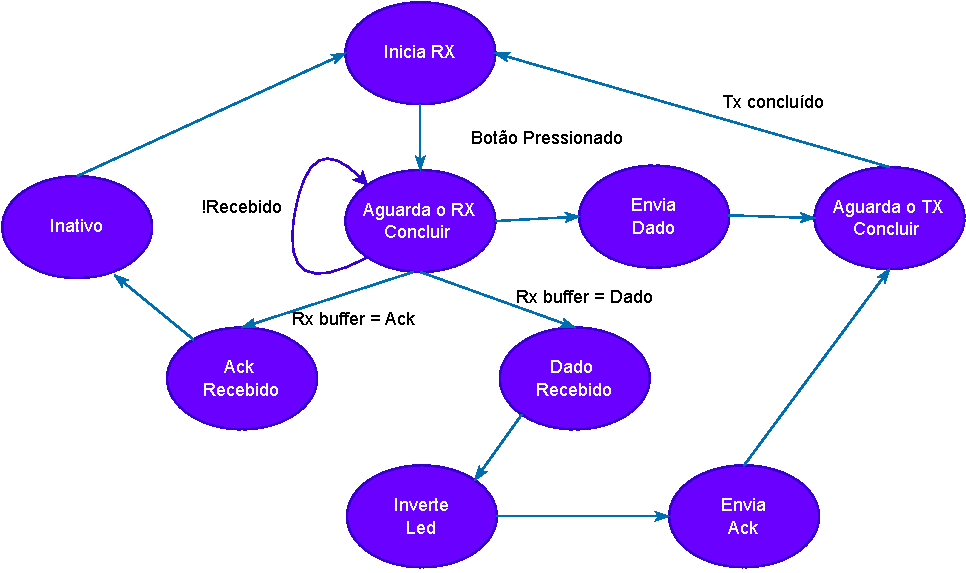
\includegraphics[scale=0.8]{img/p2p_fsm.drawio-1.pdf}
  \end{center}
    \fonte{Adaptado de \citeonline{HTSXMO32L}}
  \label{fig:p2p}
\end{figure}
%%%%%\Floatbarrier

Este algoritmo basicamente mantém o seu rádio receptor sempre ativo e é capaz de ligar o transmissor a qualquer momento a partir de um evento de botão. Dentre as alterações necessárias para operação de acordo com este trabalho, destaca-se a alteração da funcionalidade do botão para simular eventos do sistema de \textit{Wake-up Receiver}. Desta forma, pode-se medir a quantidade de energia dos seguintes estados de operação:
\begin{itemize}
    \item Consumo durante a transmissão de dados
    \item Consumo para escrita na memória
    \item Consumo para conversa com o RTC
    \item Consumo para leitura de tensão do super capacitor
\end{itemize}

Estas medições podem ser vistas na seção~\ref{sec:desmpenho} com uma separação de cada etapa através da sinalização do Led $D3$ que foi desabilitado através do \textit{Jumper} $JP3$, porém suas funções de acesso foram reaproveitadas para executar marcações monitoradas em um canal do osciloscópio.

Com isso, desenvolveu-se duas bibliotecas para operação do sistema em linguagem C. Sendo a primeira para interface com o RTC e a segunda para acumular funções básicas descritas na lista acima. Ambas disponíveis em um repositório digital público disponibilizado pelo autor~\citeonline{repositorio} no \textit{Branch} \textit{"master\_2"}.

\subsection{Biblioteca para o RTC - RV\_3032.h}
O dispositivo de RTC escolhido para a aplicação, conta com uma interface de comunicação I$^2$C. Esta conexão não está configurada no \textit{firmware} de exemplo fornecido pela HT Micron, porém a adição desse recurso pode ser incluída através da interface de configuração Cube MX que é a solução disponibilizada para pré configuração do microcontrolador em projetos de software.
Após essa configuração da comunicação I$^2$C, se fez necessário o desenvolvimento de uma biblioteca de funções de acesso para as configurações disponíveis no RTC.
Para tal, se usou como referência o driver~\cite{rtcdriver} para Linux oferecido pelo fabricante do RTC através de cadastro prévio para execução de download. 

A partir dai, utilizou-se as funções de comunicação I$^2$C geradas pelo Cube MX para interfacear as funções do RTC através das funções \textit{"HAL\_I2C\_Master\_Transmit"} e \textit{"HAL\_I2C\_\_Master\_Receive"}. Para o mapeamento de instruções com seus respectivos endereços, montou-se uma sequência de \textit{"\#define"} conforme a documentação do RTC. Cabe um destaque especial para as principais funções utilizadas, embora a biblioteca gerada possua outros recursos dispensáveis a este projeto.
\begin{itemize}
    \item \textit{updateTime} - Consulta a hora e dia no RTC pela I$^2$C;
    \item \textit{getEpoch} - Transforma as variáveis de tempo em \textit{Timestamp};
    \item \textit{getTemperature} - Consulta a temperatura no RTC pela I$^2$C;
    \item \textit{readRegister} - Interface de leitura com a biblioteca I$^2$C do Cube IDE;
    \item \textit{writeRegister} - Interface de escrita com a biblioteca I$^2$C do Cube IDE;
\end{itemize}

\subsection{Biblioteca para funções básicas - TCC.h}
Para as demais operações, inclusive de interfaceamento entre a biblioteca do RTC produzida e citada acima, desenvolveu-se uma série de funções para acumular rotinas mais extensas, tornando assim o código na função principal do sistema contida no arquivo \textit{"main.c"} organizada e de fácil entendimento.

\begin{itemize}
    \item \textit{TCC\_Radio} - Configura o Rádio;
    \item \textit{TCC\_Transmit} - Transmite os dados por RF;
    \item \textit{TCC\_Recive} - Recebe dados por RF;
    \item \textit{\_printbits} - Auxilia na visualização de variáveis binárias;
    \item \textit{clearData} - Limpa a Memória de dados armazenados;
    \item \textit{saveData} - Salva o dado coletado na memória;
    \item \textit{printMemory} - Auxilia na depuração dos dados coletados;
    \item \textit{readVoltage} - Lê a tensão atual do super capacitor;
\end{itemize}

\subsubsection{Leitura da tensão do super capacitor}
Outro recurso igualmente adicionada no \textit{firmware} através da interface de configuração do Cube MX foi a leitura analógica para detecção do nível de bateria. Esta leitura leva em consideração os resistores escolhidos para compor o divisor de tensão presente no esquema elétrico da Figura~\ref{fig:esquemaEle} da seção~\ref{sec:esquematico}. Este valor obtido através do conversor A/D contendo um resultado de 12 bits, sendo o valor máximo 4095 que  pode ser entendido como a tensão máxima do microcontrolador que é de 3,3 V. Devido a relação do divisor de tensão presente no circuito, esse valor de 4095 representa para o super capacitor uma tensão de 5,58 V.

\subsubsection{Organização da memória}
O microcontrolador presente no sistema possui uma memória disponível para alocação de dois mil dados de 8 bits. O dado de temperatura armazenado na memória pode ser escrito com apenas 8 bits abrangendo uma faixa que compreende de -128~$^o$C até 127~$^o$C. Já o a informação de tempo, originalmente ela contém 32 bits e representa todos os segundos desde o dia primeiro de janeiro de 1970 até as 6:28 do dia 7 de fevereiro de 2106. Entretanto, devido a uma característica do sistema de privilegiar a maior quantidade de coletas de temperatura, fez-se um equilíbrio entre a quantidade de medidas de tempo necessárias e a quantidade de memória disponível. Considerando empiricamente um intervalo de tempo de aproximadamente 20 dias em um espaço de tempo de 1 hora entre cada medição de temperatura, pode-se esperar 480 medições. Dividindo o espaço da memória de 2000 por 480 se chega a um total de 4 bytes para armazenamento da informação. Reservando um byte para a informação de temperatura, sobram 3 bytes para a informação de tempo. Nesse momento se fez uma escolha para reduzir o intervalo de tempo do \textit{"Timestamp"} de 1 segundo para 4 minutos e 15 segundos aplicando uma máscara nos 8 bits menos significativos da informação de tempo. Com isso, apesar de se ter uma variação considerável de tempo no momento exato da medição, não se tem um prejuízo significativo com o dado que se espera coletar, visto que o intervalo de medição é de 1 hora.

Além do dado de temperatura e tempo, se fez necessário a ocupação de uma posição da memória para armazenar um indexador de valores salvos. Para isso, reservou-se os primeiros 4 bytes da memória. Sendo assim, a quantidade de informações de tempo e temperatura pode ser calculado na equação~\ref{equ:memoria} onde se chegou a um total de 499 posições disponíveis para salvar os dados coletados.

\begin{equation}
    \label{equ:memoria}
    Quantidade~Dados = \frac{2~kbytes}{4} - 4\times(indexador) = 499~dados
\end{equation}


%%%%%%%%%%%%%%%%%%%%%%%%%%%%%%%%%%%%%%%%%%%%%%%%%%%%%%%%%%%%%%%%%%%%%%
 
%%%%%%%%%%%%%%%%%%%%%%%%%%%%%%%%%%%%%%%%%%%%%%%%%%%%%%%%%%%%%%%%%%%%%%
\section{Desempenho energético}\label{sec:desmpenho}
%%%%%%%%%%%%%%%%%%%%%%%%%%%%%%%%%%%%%%%%%%%%%%%%%%%%%%%%%%%%%%%%%%%%%%
De modo a avaliar o comportamento de todos os dispositivos eletrônicos ligados ao sistema de alimentação, produziu-se a tabela contendo os principais componentes de hardware ligados à alimentação principal do sistema. Na Tabela~\ref{tab:devicelist} é possível ver a lista de dispositivos, bem como suas principais características elétricas.


\begin{table}[]
\caption{Relação consumo teórico dos dispositivos do sistema}
  \label{tab:devicelist}
\begin{tabular}{lll}
\hline
\textbf{Descrição}  & \textbf{Código} & \textbf{Características}                  \\ \hline
Microcontrolador    & iMCP HT32SX     & TX \IradioTX; RX \IradioRX; Standaby 1~mA \\
RTC Micro Crystal   & RV3032          & I \IRTC; Vmin \VminRTC                \\
Regulador LDO       & TLV758P         & Dropout \DropV; Iq 25~μA; Max 500~mA      \\
Led Power           & IN-S63AT5B      & Vf 2,8V; I 5mA                            \\
Super Capacitor     & LM055224A       & C 0,22~F; ESR 6 ~ \ESRmax ; Fuga 0,5~10μ A\\ \hline
\end{tabular}
\fonte{Elaborado pelo autor}
\end{table}

Para uma avaliação de consumo energético, levou-se em consideração três cenários distintos. O primeiro deles avaliando o consumo do único dispositivo (RTC) ligado constantemente ao super capacitor. O segundo cenário, considerando apenas o consumo do módulo iMCP HTSXMO32L-22 executando tarefa básicas e com transmissão de RF. E um último cenário uma avaliação do desempenho considerando o uso das funções básicas independente da transmissão onde o dispositivo se torna um \textit{Datalogger} durante a maior parte do tempo e um transmissor contínuo de RF descarregamento dos dados armazenados no trajeto.


\subsection{Consumo do RTC}
A partir do gráfico da Figura~\ref{fig:capdescargaT}, pode-se inspecionar visualmente o tempo de descarga do circuito em duas etapas. Inicialmente desconsiderando a corrente do circuito da placa iMCP HTSXMO32L-22. Esta inferência pode ser feita, calculando uma impedância padrão apenas para a corrente do circuito do RTC. A Tabela~\ref{tb:RTC} contém os dados teóricos ($I_{RTC}$ e $V_{min}$) e práticos ($V_{cc}$ e $V_{diodo}$) obtidos através de medições em laboratório. Através destes dados se pode estimar na equação~\ref{equ:zRTC} a resistência constante estimada de carga do RTC.

\begin{table}
\begin{center}
\caption{Características Elétricas do RTC}
\label{tb:RTC}
\begin{tabular}{@{}cccc@{}}
\toprule
\textbf{Descrição} & \textbf{Nome}                  &\textbf{Valor} \\ \midrule
$I_{RTC}$   & Corrente nominal do RTC               & \IRTC       \\
$V_{min}$   & Tensão mínima de funcionamento do RTC & \VminRTC        \\
$V_{cc}$    & Tensão de Entrada                     & \Vcc         \\
$V_{diodo}$ & Queda de tensão do diodo              & \Vdiodo      \\ \bottomrule
\end{tabular}
\end{center}  
\fonte{Elaborado pelo autor}
\end{table}

\begin{equation}
    R_{L} = \frac{V_{cc}-V_{diodo}}{I_{RTC}} = \frac{\Vcc-\Vdiodo}{\IRTC} = \LRTCb
  \label{equ:zRTC}
\end{equation}

Uma vez que está resistência constante estimada de carga esteja mapeada, pode-se observar o gráfico da Figura~\ref{fig:capdescargaT} que apresenta 4 linhas de descarga a partir do potencial de 5V. Entretanto, a tensão máxima disponível máxima deve considerar a queda de tensão no diodo em série com o super capacitor. Logo essa tensão será de \Vcap. Como as operações do RTC são garantidas até a tensão de \VminRTC, pode-se inferir um tempo de operação apenas com o RTC ligado ao circuito de 550~horas ou 22,9 dias. Essa análise toma como base a curva de 5~M$\Omega$ para uma carga constante em 25~$^o$C. Na falta de uma curva caracterizada pelo fabricante do capacitor para \LRTC, esse curva pode ser tomada como uma aproximação teórica mais adequada que a apresentada na Figura~\ref{fig:capdescargaT}, sendo necessária uma análise prática posterior para obter o tempo real. Esse resultado destoa do esperado na seção~\ref{sec:supercap} onde se esperava uma duração de 40~dias na equação~\ref{eq:T} devido à corrente de fuga desconsiderada na ocasião desta avaliação.


\begin{figure}[h!]
  \caption{Curva de descarga do capacitor de acordo com o datasheet.}
  \begin{center}
      \includegraphics[page=9,scale=2,
      %trim={<left> <lower> <right> <upper>} 
      trim={15.5cm 5.6cm 1.5cm 19cm},
      clip]{Anexo/cap_max.pdf}
  \end{center}
  \fonte{\citeonline[p.~9]{Ohmite}}
  \label{fig:capdescargaT}
\end{figure}
%%%%%\Floatbarrier


\subsection{Consumo do iMCP HTSXMO32L-22}

Uma vez que esse trabalho se dispõe a gerenciar a alimentação de modo possibilitar distribuição de energia apenas por um super capacitor, pode-se verificar que o principal consumidor de energia do sistema é o microcontrolador. Embora se tenha estabelecido na seção~\ref{sec:esquematico} que este ficará desligado todo o tempo, há de se levar em consideração a corrente de consumo em modo de transmissão (TX) que é da ordem de \IradioTX. Esse nível de corrente é impraticável para o supercapacitor que possui uma ESR (resistência série equivalente) típica de até \ESRmax. Com isso, pode-se calcular a queda de tensão máxima no circuito com essa resistência na equação~\ref{equ:esrqueda}.

\begin{equation}
    V_{queda} = I_{max}\times ESR = \IradioTX \times \ESRmaxb = \Vqueda
  \label{equ:esrqueda}
\end{equation}

Com essa diferença de tensão na entrada se somando ao \textit{Dropout} de \DropV, tem-se uma tensão máxima na saída do regulador de tensão de \VoutMin, sendo esta inferior aos \VmcuMin requeridos para o funcionamento do HT32SX. Com isso, pode-se convencionar uma corrente máxima para esta potência, considerando a capacidade disponível no super capacitor escolhido obtendo primeiramente a queda máxima de tensão na equação~\ref{equ:Vfunc} e calculando essa corrente na equação~\ref{equ:ifunc}.

\begin{equation}
   V_{funcional de queda} =  V_{cap} - V_{MCU} = \Vcap - \VmcuMin = \VquedaFun
  \label{equ:Vfunc}
\end{equation}

\begin{equation}
   I_{funcional} = \frac{V_{funcional de queda}}{ESR} = \frac{\VquedaFun}{\ESRmaxb} = \ImaxCap
  \label{equ:ifunc}
\end{equation}

Entretanto, o rádio interno do HT32SX, possui outros modos de operação em que é possível reduzir os níveis de corrente apenas desligando o \textit{Power Amplifier} (PA) do rádio. Este modo de operação é chamado de \textit{"PA SHUTDOWN"} pelo fabricante do microcontrolador em sua documentação de \textit{software}. Além do desligamento do PA, este ainda pode ser configurado para operar com desvio ao que o fabricante atribuiu o nome de \textit{"PA BY PASS"}. Já o modo com potência máxima é atribuído o nome de \textit{"PA TX"} que é destinado a operações de comunicação em longas distâncias. Embora este modo de operação seja uma funcionalidade interessante para o acompanhamento em tempo real da temperatura de uma determinada carga de alimentos através da infraestrutura de rede instalada de Sigfox no mundo, ele não se faz necessário, visto que a curva de temperatura pode ser armazenada na memória e obtida através de um dispositivo de coleta de dados especial no destino final da carga ou em pontos intermediários preparados para isso.

Com tudo, de forma a comparar os três modos de operação, optou-se por testar ambas e observar seus resultados que seguem nas figuras~\ref{fig:PA_TX}, \ref{fig:PA_SHUTDOWN} e \ref{fig:PA_BY_PASS}. Nestes gráficos podem ser observados a identificação de cada etapa do processo elaborado pelo autor no dedicado que foi gravado no microcontrolador. Cada etapa foi sinalizada com um pino auxiliar de GPIO do próprio HT32SX. O monitoramento da corrente foi executado com o auxílio de um resistor de baixa resistência, tipicamente chamado de \textit{Shunt}, para acompanhar a queda de tensão sobre este. Este resistor foi aplicado na entrada da alimentação do regulador de tensão e detecta a corrente consumida do super capacitor pelo sistema. As cinco principais etapas do algoritmo podem ser vistas com cores diferentes nos gráficos indicados. Além dessa informação visual, devido ao processo de aquisição desta corrente com a captura de pontos e arquivo CSV (Valores separados por vírgula) gerado pelo osciloscópio utilizado no processo de depuração. Com isso, esses sinais puderam ser integrados e exibidos nas tabelas~\ref{tab:PA_TX}, \ref{tab:PA_SHUTDOWN}, \ref{tab:PA_BY_PASS} e \ref{tab:PA_RX}.


\begin{figure}[h!]
  \caption{Corrente de alimentação em modo PA TX.}
  \begin{center}
      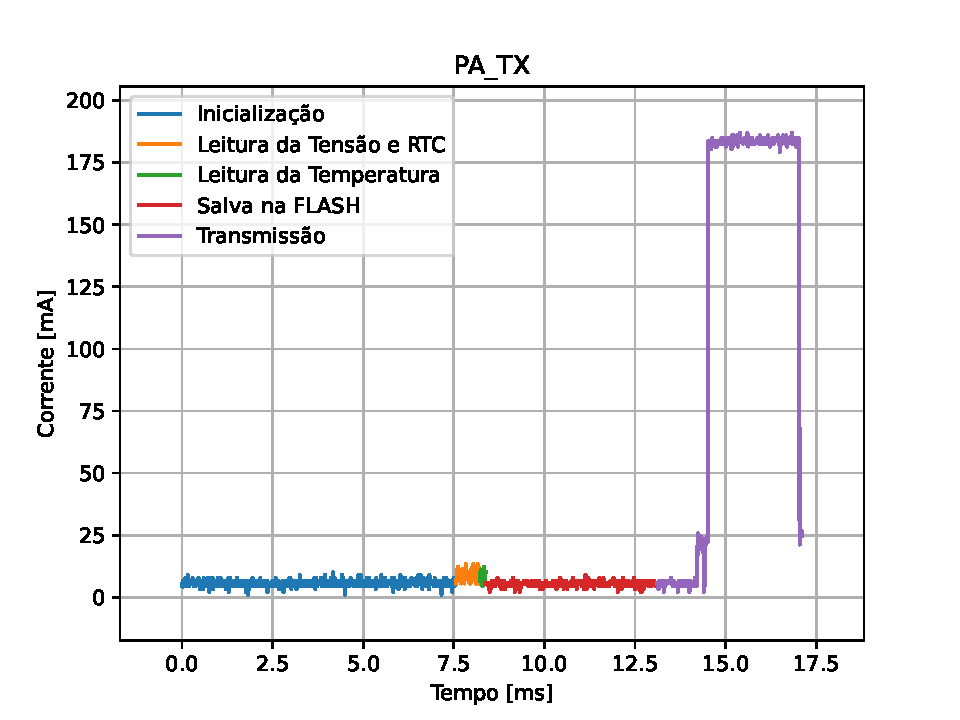
\includegraphics[scale=0.8]{scripts/PA_TX.pdf}
  \end{center}
  \fonte{Elaborado pelo autor}
  \label{fig:PA_TX}
\end{figure}
%%%%%\Floatbarrier

\input{scripts/Tabelas/TabelaPA_TX}

Já na Figura~\ref{fig:PA_TX} pode ser observado que mesmo na menor opção de potência do rádio da ordem de 12~dBm e com o desligamento do sistema de \textit{Booster}, a corrente máxima da entrada durante o processo de transmissão ultrapassa os \ImaxCap disponíveis pelo super capacitor.


\begin{figure}[h!]
  \caption{Corrente de alimentação em modo PA SHUTDOWN.}
  \begin{center}
      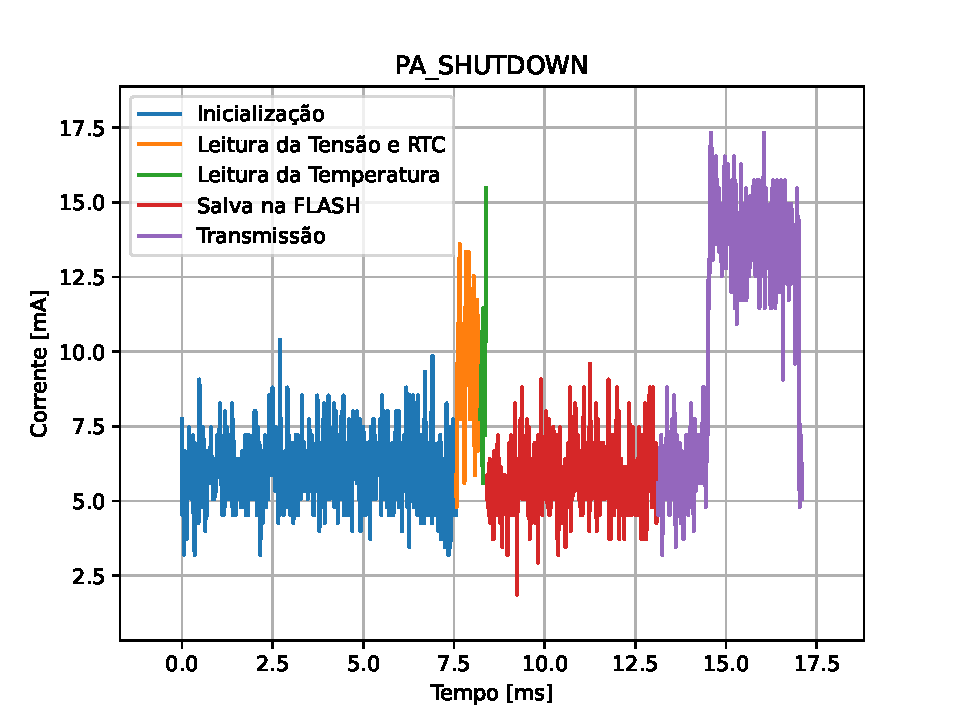
\includegraphics[scale=0.8]{scripts/PA_SHUTDOWN.pdf}
  \end{center}
  \fonte{Elaborado pelo autor}
  \label{fig:PA_SHUTDOWN}
\end{figure}
%%%%%\Floatbarrier

\input{scripts/Tabelas/TabelaPA_SHUTDOWN}


\begin{figure}[h!]
  \caption{Corrente de alimentação em modo PA BY PASS.}
  \begin{center}
      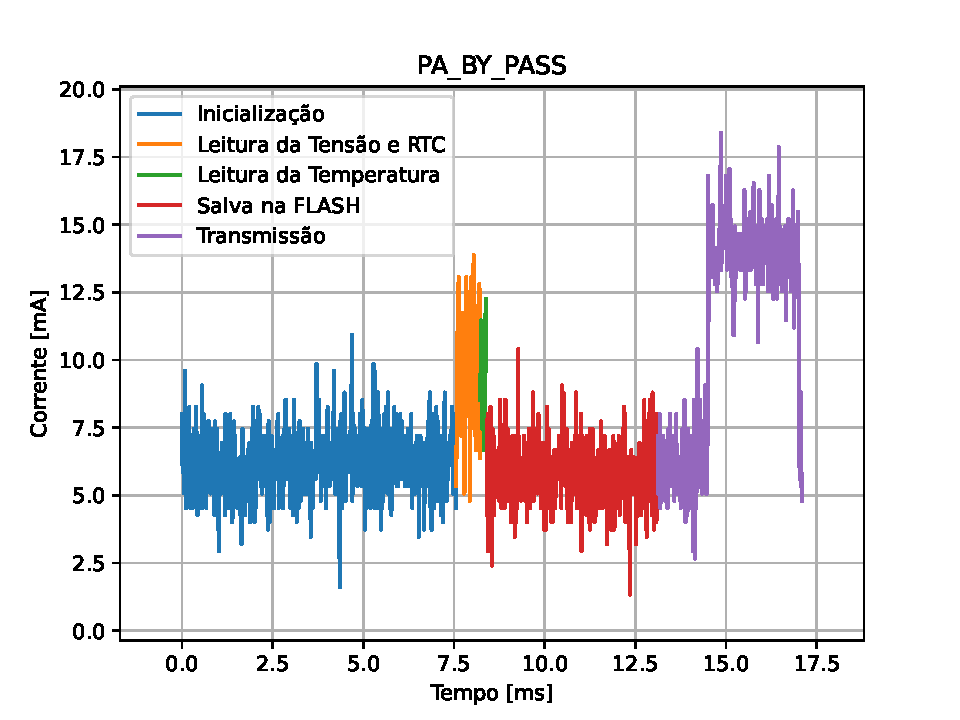
\includegraphics[scale=0.8]{scripts/PA_BY_PASS.pdf}
  \end{center}
  \fonte{Elaborado pelo autor}
  \label{fig:PA_BY_PASS}
\end{figure}
%%%%%\Floatbarrier

\input{scripts/Tabelas/TabelaPA_BY_PASS}

Conforme o esperado, a única diferença significativa de consumo ocorre entre o modo \textit{"PA TX"} e os demais. Com uma aproximação muito grande entre os modos \textit{"PA SHUTDOWN"} e \textit{"PA BY PASS"}. Além disso, nas tabelas também é possível observar que a maior corrente nesses dois modos não passa de 20~mA que é muito abaixo do limite máximo de \ImaxCap~estabelecido na equação~\ref{equ:ifunc}.





Considerando que a memória disponível para armazenamento discutida na seção~\ref{sec:software} será de 499 dados, pode-se testar a efetividade desta aplicação executando 499 ligamentos no microcontrolador e executando todos os passos esperados em um uso normal.
\begin{enumerate}
    \item Inicialização do microcontrolador;
    \item Medir o nível de tensão do super capacitor;
    \item Consultar o \textit{"Timestamp"} atual no RTC;
    \item Medir a temperatura;
    \item Ler a memória para verificar onde salvar o próximo dado;
    \item Salvar os dados na memória flash do microcontrolador;
    \item Realizar uma transmissão de RF;
    \item Desligar o pino que mantém o microcontrolador alimentado;
\end{enumerate}

Após esse teste, notou-se que o nível de alimentação do super capacitor que inicialmente estava com \Vcap, teve uma redução de 300~mV que representa uma redução de 25~horas se tomar como base o gráfico da Figura~\ref{fig:capdescargaT}. Em linhas gerais se pode dizer o processo de transmissão completa da memória gasta o equivalente a 1~dia.




\subsection{Perfil de consumo baseado em tarefas distintas}
A partir deste ponto, se pode especular com mais propriedade o modo de operação definido para este sistema. Tomando como base a premissa de garantia de aquisição dos dados e sabendo que as perdas de dados em zonas de sombra da rede Sigfox implantada, percebe-se que o envio constante de dados pode servir a um outro propósito, mas não para garantia dos dados. Sendo assim, a ideia de privilegiar o consumo de corrente apenas para as operações de salvamento de dados na memória do microcontrolador aparenta ser a melhor solução. Já para aquisição de dados coletados, pode-se produzir um dispositivo de coleta dedicado a receber os dados armazenados sem uma preocupação com o dispositivo atingir níveis críticos de alimentação do super capacitor, pois os dados estão retidos na memória, bastando apenas um carregamento pelo sistema de colheita de energia para efetuar uma transmissão completa. Neste cenário, o dispositivo ganha 1~dia de energia para outras operações.



\subsection{Perfil de consumo no modo de escuta}
Em uma última análise, mediu-se o desempenho energético em modo de configuração, onde o dispositivo seria acordado por um sistema de \textit{"Wake-up Receiver"}, entraria em modo de recepção, recebendo frame e respondendo uma confirmação para garantir a correta configuração.Na Figura~\ref{fig:PA_RX} pode ser observado que o embora o consumo seja relativamente baixo na hora da recepção, o tempo necessário para isso faz com que a energia utilizada atinja patamares na ordem de 2,5~J.

Para distinguir os modos de operação, basta que o sistema de \textit{"Wake-up Receiver"} ative um dos pinos de GPIO do microcontrolador que originalmente era destinado ao botão do usuário, possibilitando assim que este opere de modo a transmitir todos os dados da memória juntamente com o número de coletas executadas para que se possa fazer uma checagem quanto ao recebimento total de dados da memória.


\begin{figure}[h!]
  \caption{Corrente de alimentação em modo PA RX.}
  \begin{center}
      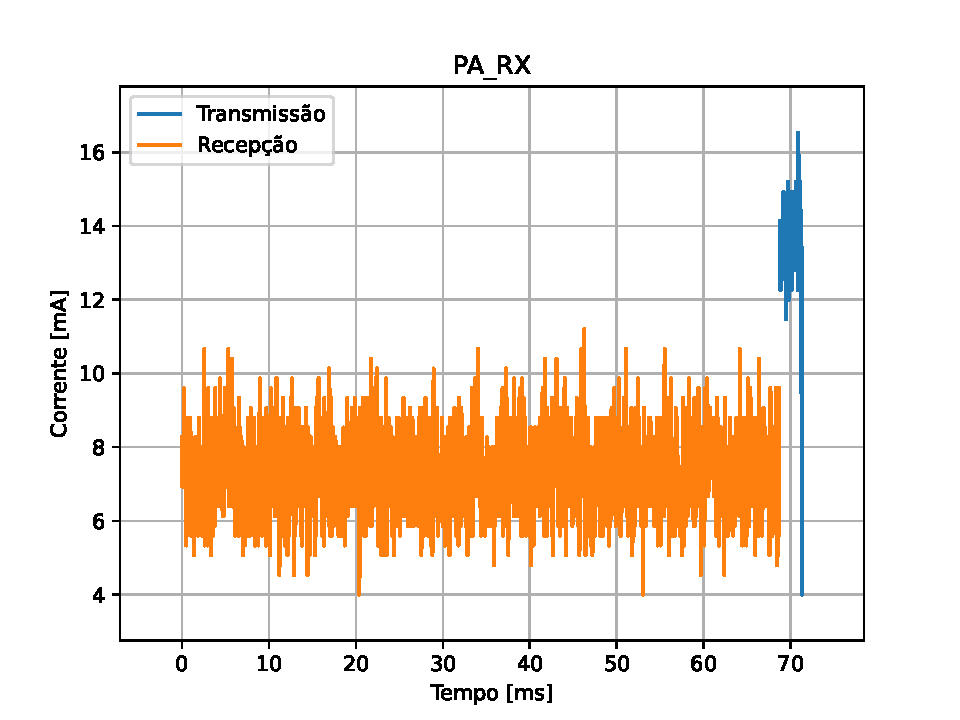
\includegraphics[scale=0.8]{scripts/PA_RX.pdf}
  \end{center}
  \fonte{Elaborado pelo autor}
  \label{fig:PA_RX}
\end{figure}
%%%%%\Floatbarrier

\input{scripts/Tabelas/TabelaPA_RX}

%%%%%%%%%%%%%%%%%%%%%%%%%%%%%%%%%%%%%%%%%%%%%%%%%%%%%%%%%%%%%%%%%%%%%%
\section{Análise dos resultados}
%%%%%%%%%%%%%%%%%%%%%%%%%%%%%%%%%%%%%%%%%%%%%%%%%%%%%%%%%%%%%%%%%%%%%%
Considerando os fatores que levaram em conta a escolha do protocolo Sigfox para a rede de comunicação de RF, pode-se dizer que a disponibilidade de infraestrutura no mundo passa por uma incerteza devido a uma possível falência desta empresa. Entretanto, devido a forma como o projeto foi concebido, com algumas alterações pontuais é possível migrar para outro dispositivo com características semelhantes.

Quanto a escolha do RTC e seu desempenho funcional, pode-se notar que o resultado prático se manteve dentro da especificação. Combinado com o super capacitor, este dispositivo possibilita um tempo de utilização sem bateria suficiente para cobrir o transporte de alimentos mesmo em países com dimensões continentais como o Brasil.

Já a especificação do microcontrolador com rádio, além das limitações de uma possível falta de cobertura da rede Sigfox, ainda precisou ter sua potência reduzida com o desligamento do amplificado de potência do rádio. Isso não significa necessidade de mudança para outro sistema de alimentação ou de rede, mas serve como sinalização para trabalhos futuros que utilizem esta forma de alimentação por super capacitor.

Quanto as rotinas de software, percebeu-se que além do já esperado consumo alto das atividades que envolvem a transmissão de rádio, pode-se observar que a quantidade de energia da inicialização do microcontrolador representaram um elevado consumo que superou a energia de uma transmissão de rádio (considerando o amplificado de potência desligado). Em terceiro lugar o salvamento de dados na memória do microcontrolador que assim como a inicialização, apresentam esse consumo elevado devido ao tempo necessário para realizar suas tarefas.

Todos os testes de desempenho energético foram realizados com o auxilio de um osciloscópio para captura dos sinais e de um multímetro, além do uso de um analisador lógico para desenvolvimento e testes de depuração da comunicação I$^2$C do microcontrolador com o RTC. O ambiente de testes pode ser visto na Figura~\ref{fig:setup}

\begin{figure}[h!]
  \caption{Local de testes e equipamentos usados.}
  \begin{center}
      \includegraphics[scale=0.1]{img/setup.png}
  \end{center}
  \fonte{Elaborado pelo autor}
  \label{fig:setup}
\end{figure}
%%%%%\Floatbarrier

Talvez o resultado mais surpreendente em termos de consumo energético se deu em função do modo de recepção de rádio, visto que o tempo necessário para evitar uma colisão da confirmação de resposta é consideravelmente alto. Uma alternativa para resolver esse problema de gasto energético seria o desligamento da confirmação de resposta, mas isso implicaria na incerteza de configuração do dispositivo e portanto deve ser mantido.

Quanto a autonomia foi possível atingir um total de 20 dias sem a necessidade de carregamento externo e ainda conseguindo: ler, gravar e transmitir 499 dados coletados.